% Options for packages loaded elsewhere
\PassOptionsToPackage{unicode}{hyperref}
\PassOptionsToPackage{hyphens}{url}
\PassOptionsToPackage{dvipsnames,svgnames,x11names}{xcolor}
%
\documentclass[
  12pt,
]{report}

\usepackage{amsmath,amssymb}
\usepackage{setspace}
\usepackage{iftex}
\ifPDFTeX
  \usepackage[T1]{fontenc}
  \usepackage[utf8]{inputenc}
  \usepackage{textcomp} % provide euro and other symbols
\else % if luatex or xetex
  \usepackage{unicode-math}
  \defaultfontfeatures{Scale=MatchLowercase}
  \defaultfontfeatures[\rmfamily]{Ligatures=TeX,Scale=1}
\fi
\usepackage{lmodern}
\ifPDFTeX\else  
    % xetex/luatex font selection
    \setmainfont[]{Times New Roman}
    \setsansfont[]{Arial}
    \setmonofont[]{Courier New}
\fi
% Use upquote if available, for straight quotes in verbatim environments
\IfFileExists{upquote.sty}{\usepackage{upquote}}{}
\IfFileExists{microtype.sty}{% use microtype if available
  \usepackage[]{microtype}
  \UseMicrotypeSet[protrusion]{basicmath} % disable protrusion for tt fonts
}{}
\usepackage{xcolor}
\usepackage[top=30mm,left=1in,right=1in,bottom=25mm,top = 3cm,bottom =
3cm,left = 3cm,right = 2.7cm]{geometry}
\setlength{\emergencystretch}{3em} % prevent overfull lines
\setcounter{secnumdepth}{5}
% Make \paragraph and \subparagraph free-standing
\makeatletter
\ifx\paragraph\undefined\else
  \let\oldparagraph\paragraph
  \renewcommand{\paragraph}{
    \@ifstar
      \xxxParagraphStar
      \xxxParagraphNoStar
  }
  \newcommand{\xxxParagraphStar}[1]{\oldparagraph*{#1}\mbox{}}
  \newcommand{\xxxParagraphNoStar}[1]{\oldparagraph{#1}\mbox{}}
\fi
\ifx\subparagraph\undefined\else
  \let\oldsubparagraph\subparagraph
  \renewcommand{\subparagraph}{
    \@ifstar
      \xxxSubParagraphStar
      \xxxSubParagraphNoStar
  }
  \newcommand{\xxxSubParagraphStar}[1]{\oldsubparagraph*{#1}\mbox{}}
  \newcommand{\xxxSubParagraphNoStar}[1]{\oldsubparagraph{#1}\mbox{}}
\fi
\makeatother


\providecommand{\tightlist}{%
  \setlength{\itemsep}{0pt}\setlength{\parskip}{0pt}}\usepackage{longtable,booktabs,array}
\usepackage{calc} % for calculating minipage widths
% Correct order of tables after \paragraph or \subparagraph
\usepackage{etoolbox}
\makeatletter
\patchcmd\longtable{\par}{\if@noskipsec\mbox{}\fi\par}{}{}
\makeatother
% Allow footnotes in longtable head/foot
\IfFileExists{footnotehyper.sty}{\usepackage{footnotehyper}}{\usepackage{footnote}}
\makesavenoteenv{longtable}
\usepackage{graphicx}
\makeatletter
\def\maxwidth{\ifdim\Gin@nat@width>\linewidth\linewidth\else\Gin@nat@width\fi}
\def\maxheight{\ifdim\Gin@nat@height>\textheight\textheight\else\Gin@nat@height\fi}
\makeatother
% Scale images if necessary, so that they will not overflow the page
% margins by default, and it is still possible to overwrite the defaults
% using explicit options in \includegraphics[width, height, ...]{}
\setkeys{Gin}{width=\maxwidth,height=\maxheight,keepaspectratio}
% Set default figure placement to htbp
\makeatletter
\def\fps@figure{htbp}
\makeatother
% definitions for citeproc citations
\NewDocumentCommand\citeproctext{}{}
\NewDocumentCommand\citeproc{mm}{%
  \begingroup\def\citeproctext{#2}\cite{#1}\endgroup}
\makeatletter
 % allow citations to break across lines
 \let\@cite@ofmt\@firstofone
 % avoid brackets around text for \cite:
 \def\@biblabel#1{}
 \def\@cite#1#2{{#1\if@tempswa , #2\fi}}
\makeatother
\newlength{\cslhangindent}
\setlength{\cslhangindent}{1.5em}
\newlength{\csllabelwidth}
\setlength{\csllabelwidth}{3em}
\newenvironment{CSLReferences}[2] % #1 hanging-indent, #2 entry-spacing
 {\begin{list}{}{%
  \setlength{\itemindent}{0pt}
  \setlength{\leftmargin}{0pt}
  \setlength{\parsep}{0pt}
  % turn on hanging indent if param 1 is 1
  \ifodd #1
   \setlength{\leftmargin}{\cslhangindent}
   \setlength{\itemindent}{-1\cslhangindent}
  \fi
  % set entry spacing
  \setlength{\itemsep}{#2\baselineskip}}}
 {\end{list}}
\usepackage{calc}
\newcommand{\CSLBlock}[1]{\hfill\break\parbox[t]{\linewidth}{\strut\ignorespaces#1\strut}}
\newcommand{\CSLLeftMargin}[1]{\parbox[t]{\csllabelwidth}{\strut#1\strut}}
\newcommand{\CSLRightInline}[1]{\parbox[t]{\linewidth - \csllabelwidth}{\strut#1\strut}}
\newcommand{\CSLIndent}[1]{\hspace{\cslhangindent}#1}

\usepackage{booktabs}
\usepackage{caption}
\usepackage{longtable}
\usepackage{colortbl}
\usepackage{array}
\usepackage{anyfontsize}
\usepackage{multirow}
\usepackage{sectsty}
\chapterfont{\centering}
\usepackage{lscape}
\newcommand{\blandscape}{\begin{landscape}}
\newcommand{\elandscape}{\end{landscape}}
\makeatletter
\@ifpackageloaded{caption}{}{\usepackage{caption}}
\AtBeginDocument{%
\ifdefined\contentsname
  \renewcommand*\contentsname{Table of contents}
\else
  \newcommand\contentsname{Table of contents}
\fi
\ifdefined\listfigurename
  \renewcommand*\listfigurename{Figures}
\else
  \newcommand\listfigurename{Figures}
\fi
\ifdefined\listtablename
  \renewcommand*\listtablename{Tables}
\else
  \newcommand\listtablename{Tables}
\fi
\ifdefined\figurename
  \renewcommand*\figurename{Figure}
\else
  \newcommand\figurename{Figure}
\fi
\ifdefined\tablename
  \renewcommand*\tablename{Table}
\else
  \newcommand\tablename{Table}
\fi
}
\@ifpackageloaded{float}{}{\usepackage{float}}
\floatstyle{ruled}
\@ifundefined{c@chapter}{\newfloat{codelisting}{h}{lop}}{\newfloat{codelisting}{h}{lop}[chapter]}
\floatname{codelisting}{Listing}
\newcommand*\listoflistings{\listof{codelisting}{List of Listings}}
\makeatother
\makeatletter
\makeatother
\makeatletter
\@ifpackageloaded{caption}{}{\usepackage{caption}}
\@ifpackageloaded{subcaption}{}{\usepackage{subcaption}}
\makeatother

\ifLuaTeX
  \usepackage{selnolig}  % disable illegal ligatures
\fi
\usepackage{bookmark}

\IfFileExists{xurl.sty}{\usepackage{xurl}}{} % add URL line breaks if available
\urlstyle{same} % disable monospaced font for URLs
\hypersetup{
  pdftitle={Leadership Transitions and Survival: Coups, Autocoups, and Power Dynamics},
  pdfauthor={Zhu Qi},
  colorlinks=true,
  linkcolor={blue},
  filecolor={Maroon},
  citecolor={Blue},
  urlcolor={blue},
  pdfcreator={LaTeX via pandoc}}


\title{Leadership Transitions and Survival: Coups, Autocoups, and Power
Dynamics}
\author{Zhu Qi}
\date{}

\begin{document}


\def\spacingset#1{\renewcommand{\baselinestretch}%
{#1}\small\normalsize} \spacingset{1}


%%%%%%%%%%%%%%%%%%%%%%%%%%%%%%%%%%%%%%%%%%%%%%%%%%%%%%%%%%%%%%%%%%%%%%%%%%%%%%

\title{\bf Leadership Transitions and Survival: Coups, Autocoups, and
Power Dynamics}
\author{
Zhu Qi\\University of
Essex\\\href{mailto:qz21485@essex.ac.uk}{qz21485@essex.ac.uk}
}

\maketitle

\bigskip
\bigskip
\begin{abstract}

\end{abstract}


\newpage
\spacingset{1.9} % DON'T change the spacing!
\renewcommand*\contentsname{Contents}
{
\hypersetup{linkcolor=}
\setcounter{tocdepth}{2}
\tableofcontents
}
\listoffigures
\listoftables

\setstretch{1.618}
\chapter*{Acknowledgements}\label{acknowledgements}
\addcontentsline{toc}{chapter}{Acknowledgements}

The completion of this thesis marks the end of a significant journey,
one filled with hard work, continuous learning, and moments of profound
joy. This dissertation would not have been possible without the support
and encouragement of numerous individuals to whom I am deeply indebted.

First and foremost, I extend my heartfelt gratitude to my esteemed
supervisor, Professor Kristian Skrede Gleditsch. His invaluable
guidance, unwavering support, and insightful feedback have been
instrumental in shaping this research. His expertise and encouragement
have truly been the cornerstone of this academic endeavor.

I am equally grateful to Professor Han Dorussen, the chair of my board
panel, for his continuous support and constructive criticism. His
thoughtful input has significantly enhanced the quality and depth of my
research.

I would like to acknowledge the vital contributions of my initial
co-supervisors, Dr.~Saurabh Pant and Professor David Siroky. Their
instruction and guidance during the early stages of my research, prior
to their departure from the University of Essex, laid a strong
foundation for this work.

This dissertation has benefited immensely from the expertise of several
esteemed scholars in the field. I am particularly indebted to Dr.~Brian
J Phillips, Dr. Prabin Khadka, and Dr.~Winnie Xia for their insightful
comments, advice, and suggestions. Their contributions have undoubtedly
enriched this research.

On a personal note, I owe a debt of gratitude to my family for their
unwavering support and love. To my beloved wife, Ji Zhi, who has been my
steadfast pillar of strength throughout this journey - your patience and
encouragement have been immeasurable. To my dear children, Siyan and
Sisheng, your joy and curiosity have been a constant source of
motivation and inspiration.

I am profoundly thankful to my father for his enduring support and
belief in my abilities. To the cherished memory of my late mother - your
love, guidance, and the values you instilled in me continue to shape my
path and inspire my endeavors. And to my three brothers, whose support
enabled me to pursue my PhD without worries - your contribution to this
achievement cannot be overstated.

While many have contributed to the success of this work, any errors or
shortcomings remain entirely my own.

\chapter*{Abstract}\label{abstract}
\addcontentsline{toc}{chapter}{Abstract}

This dissertation examines the dynamics of irregular power transitions,
specifically coups and autocoups, and their influence on leader
survival. Through a rigorous analysis of historical data, case studies,
and quantitative modeling, this dissertation contributes to the broader
understanding of political power dynamics and the intricate factors that
shape leadership survival in the wake of irregular transitions.

The study first highlights the critical role of power dynamics, shaped
by regime type, in determining coup success rates and attempt frequency.
Utilizing a double probit model with sample selection, the research
reveals that the expected chances of coup success significantly
influence coup attempts, with military regimes facing heightened
vulnerability due to their power structure.

While often understudied, autocoups are shown to have a substantial
impact on democratic backsliding. This research introduces a refined
definition of autocoups alongside a novel dataset encompassing events
from 1945 to 2023, enabling more robust quantitative analysis.

Employing survival analysis, the study compares the longevity of leaders
who rise to power through coups versus autocoups. The findings
demonstrate that coup-installed leaders face significantly shorter
tenures and higher risks of removal. This contrasts with autocoup
leaders who manipulate the system to extend their rule, suggesting the
potential for autocoups to motivate power grabs and contribute to
democratic backsliding.

This work contributes significantly to the political science literature
by:

\begin{itemize}
\item
  Defining key concepts: Establishing a clear definition of autocoups, a
  previously understudied phenomenon.
\item
  Introducing a novel dataset: Enabling researchers to conduct more
  comprehensive quantitative analyses of autocoups.
\item
  Establishing a general framework: Providing a comparative approach to
  studying both coups and autocoups, enabling analysis in a unified
  framework for these two highly relevant political events and their
  potential effects on democratic backsliding.
\end{itemize}

\textbf{\emph{Keywords:}} Coups, Autocoups, Power transitions,
Leadership survival, Democratic backsliding

\chapter{Introduction}\label{introduction}

\section{Research Question and
Context}\label{research-question-and-context}

Irregular power transitions, characterised by a disregard for
constitutional procedures, represent a critical area of study in
political science. These transitions not only disrupt established rules
but also often employ unconstitutional tactics to consolidate power
post-transition. Moreover, such events can inspire emulation among other
ambitious leaders, potentially triggering a cascade of similar actions
across different political contexts.

Despite extensive research on irregular power transitions, a fundamental
question continues to challenge political scientists:

\textbf{Why do some leaders face premature ousting while others extend
their tenure beyond constitutionally mandated limits?}

This inquiry extends to understanding the stark disparities in
leadership longevity, where some rulers maintain power for decades while
others' tenures are measured in years, months, or even days.

This dissertation focuses on this central question, aiming to provide a
comprehensive analysis dedicated to understanding:

\begin{itemize}
\item
  How leaders ascend to or overstay in power through unconstitutional
  means.
\item
  What factors determine the duration of a leader's rule following an
  irregular ascent to power.
\end{itemize}

\section{Coups and Autocoups: A Comparative Unified Framework for
Irregular Power
Transitions}\label{coups-and-autocoups-a-comparative-unified-framework-for-irregular-power-transitions}

In the study of irregular power transitions, coups have traditionally
dominated academic discourse due to their frequency and visibility.
According to the Archigos dataset (\citeproc{ref-goemans2009}{Goemans,
Gleditsch, and Chiozza 2009}), coups\footnote{According to the Archigos
  dataset, ``Removed by Military, without Foreign Support'' and
  ``Removed by Other Government Actors, without Foreign Support'' in the
  variable exitcode are classified as coups.} accounted for more than
half of the approximately 145 irregular leader exits from 1945 to 2015.
The Global Instances of Coups (GIC) dataset
(\citeproc{ref-powell2011}{J. M. Powell and Thyne 2011}) records an even
higher number, with 245 coup-related removals from 1950 to 2024.

The prevalence of coups has led to a well-established definition and
extensive research, particularly since the turn of the millennium
(\citeproc{ref-thyne2019}{C. L. Thyne and Powell 2019}). This scholarly
focus has resulted in a general consensus on the definition of coups, as
well as the development of comprehensive datasets for quantitative
analyses. While debates on the precise definition persist, most
scholars, including this study, adhere to the definition proposed by J.
M. Powell and Thyne (\citeproc{ref-powell2011}{2011}). This widely
accepted definition encompasses two fundamental elements:

\begin{itemize}
\item
  \textbf{Perpetrators and Victims}: Perpetrators of coups are elites
  within the existing power structure and the victims are incumbent
  executive leaders.
\item
  \textbf{Strategy and Aim}: The primary objective is the complete
  removal of incumbents from power.
\end{itemize}

It is important to note that this definition excludes actions that only
partially challenge the incumbent's authority or seek policy changes
without aiming for a complete transfer of power.

The scholarly consensus on coup definition has facilitated the
development of several comprehensive datasets, enabling rigorous
quantitative analyses in political science research. Notable among these
are: GIC Dataset, Cline Centre Coup d'État Project Dataset
(\citeproc{ref-peyton2024}{Peyton et al. 2024}), and Colpus Dataset
(\citeproc{ref-chin2021}{Chin, Carter, and Wright 2021}). These datasets
have become invaluable resources in political science, enabling
researchers to conduct large-scale, comparative studies on the causes,
dynamics, and consequences of coups across different political contexts
and historical periods.

However, another form of irregular power transition has been largely
overlooked in power transition studies: leaders who refuse to relinquish
power and extend their mandated terms. At least three challenges still
exist in the analyses of this type of irregular power transition:

\begin{itemize}
\item
  \textbf{Terminology}: Unlike the more widely accepted term ``coup,''
  various terms (e.g., self-coup, autogolpe, executive coup, incumbent
  takeover) are used to describe this phenomenon.
\item
  \textbf{Definition}: Existing definitions often conflate power
  expansion and power extension\footnote{The definitions and concepts of
    power expansion and power extension can often be ambiguous. In this
    study, we define power expansion as an incumbent acquiring
    additional authority from other branches or apparatuses of the
    state. Conversely, power extension refers to an incumbent prolonging
    their tenure beyond the originally mandated term in office.}. For
  instance, Maxwell A. Cameron (\citeproc{ref-cameron1998a}{1998a})
  defines an autogolpe primarily in terms of power expansion, which does
  not align with the definition of coup.
\item
  \textbf{Data}: A consensus dataset for autocoups is lacking, with
  existing datasets varying in terminology, definitions, and coverage
  years Baturo and Tolstrup (\citeproc{ref-baturo2022}{2022}).
\end{itemize}

To address this gap in the literature and provide a framework for
analysis, we propose the term ``autocoup'' to describe this type of
transition. This concept will be extensively discussed and defined in
Chapter 3, providing a basis for integrating these events into the
broader study of irregular power transitions and their impact on
political systems and leader longevity.

Analysing coups and autocoups within a unified framework is crucial for
a comprehensive understanding of irregular power transitions and leader
survival for three reasons:

\begin{itemize}
\tightlist
\item
  Both phenomena significantly influence democratic backsliding and
  represent the most frequent means of irregular power transition.
\item
  Their similar nomenclature reflects a fundamental similarity: while a
  coup aims to replace the current leader, an autocoup seeks to prevent
  the succession of a future leader.
\item
  This comparative approach will enable a more nuanced analysis of
  irregular power transitions, contributing to our understanding of
  political stability, democratic erosion, and leadership longevity in
  various regime types.
\end{itemize}

\section{Academic Contributions}\label{academic-contributions}

This study addresses a critical gap in the literature by offering a
unified framework for analysing both coups and autocoups. My
contributions are threefold:

\begin{itemize}
\tightlist
\item
  \textbf{Emphasis on Power Dynamics and Regime Types}: This study
  highlights the significant role of power dynamics, particularly the
  influence of regime types, in determining the success and frequency of
  coup attempts, underscores how the expected chances of coup success
  motivate such attempts, with military regimes being notably
  susceptible.
\item
  \textbf{Refined Definition and Novel Dataset for Autocoups}: I
  introduce a refined definition of autocoups, develop a novel dataset
  covering events from 1945 to 2024, and fill a significant gap in the
  existing literature and enable a comparative analysis with classic
  coups.
\item
  \textbf{Survival Analysis of Leaders from Different Entry Modes}: This
  research applys survival analysis to existing coup data and the new
  autocoup dataset, demonstrates how different modes of entry into power
  significantly affect leader survival, and reveals that leaders who
  come to power through coups typically have shorter tenures and face
  higher removal risks compared to those who extend their rule through
  autocoups.
\end{itemize}

These contributions collectively advance the field by providing a more
holistic understanding of irregular power transitions, offering new
tools and data for quantitative analysis of autocoups, and demonstrating
the interconnectedness of power acquisition methods and leadership
survival.

This work lays the foundation for future research on the dynamics of
political power, regime stability, and democratic backsliding, offering
both theoretical insights and practical implications for policy-makers
and scholars alike.

\section{Implications}\label{implications}

The examination of irregular power transitions provides a crucial
perspective on the interrelated phenomena of democratic backsliding,
breakdown, and autocratic intensification. The findings of this study
provide logical explanations for several political phenomena:

\begin{itemize}
\item
  \textbf{Regression of Global Democracy Levels}: This study can explain
  why global democracy levels have regressed to pre-2000 levels. For
  example, Freedom House reports an 18th consecutive year of global
  freedom decline in 2023
  (\citeproc{ref-freedomhouse2024freedom}{Freedom House 2024}).
  Irregular power transitions inevitably violate democratic or
  constitutional norms and disrupt the trajectory towards stable
  democracies or democratization from autocracies. Leaders who ascend
  through irregular means often undermine constitutional norms to seize
  or overstay in power, creating a vicious cycle of eroding democratic
  institutions.
\item
  \textbf{Within-Regime Democratic Erosion}: This study explains why
  democratic backsliding often occurs within regimes, with democracies
  becoming less liberal and autocracies becoming less competitive
  (\citeproc{ref-mechkova2017}{Mechkova, Lührmann, and Lindberg 2017}).
  This is particularly because autocoups have become more prevalent than
  traditional coups since 2000 (\citeproc{ref-bermeo2016}{Bermeo 2016}).
  Importantly, autocoups typically do not result in immediate regime
  change, contributing to the observed pattern of within-regime
  democratic erosion.
\item
  \textbf{Prevalence of Autocoups Since 2000}: This research explains
  why autocoups are more prevalent since 2000. Firstly, autocoups have a
  significantly higher probability of success compared to traditional
  coups. Additionally, even when unsuccessful, the repercussions of
  autocoups are generally less severe than those of failed traditional
  coups. Moreover, successful autocoup leaders tend to maintain power
  for substantially longer periods than leaders who enter through
  traditional coups.
\end{itemize}

\section{Overview of the Thesis}\label{overview-of-the-thesis}

This study investigates irregular power transitions and their
implications for leadership survival and democratic processes. I examine
three key aspects: classic coup attempts, autocoups, and how the method
of power acquisition impacts leader longevity.

\subsection{Chapter 2: Determinants of Classic Coup
Attempts}\label{chapter-2-determinants-of-classic-coup-attempts}

This chapter delves into the factors influencing classic coup attempts,
with a novel focus on the less observable but crucial factor of expected
coup success rates. Key features include the utilization of a double
probit model with sample selection and the analysis of how expected
success rates significantly influence coup attempts. It also examines
how regime types shape the balance of power between incumbents and
challengers, determining the chances of success of coups. Findings
indicate a substantially higher coup risk in military regimes compared
to dominant-party regimes.

\subsection{Chapter 3: Conceptualising and Analysing
Autocoups}\label{chapter-3-conceptualising-and-analysing-autocoups}

This chapter refines and analyses the concept of autocoups, with a
specific focus on power extensions by incumbent leaders. Notable
elements include the redefinition of autocoups as instances where
incumbent leaders refuse mandated power transitions. Introduction of a
novel dataset covering autocoup events from 1945 to 2024, encompassing
110 attempts and 87 successes. Presentation of case studies and
empirical analyses demonstrating the utility of this dataset for more
quantitative research in political science.

\subsection{Chapter 4: Impact of Power Acquisition Methods on Leadership
Longevity}\label{chapter-4-impact-of-power-acquisition-methods-on-leadership-longevity}

This chapter investigates how the method of power acquisition affects
the tenure of leaders who ascend through coups versus those who extend
their tenure via autocoups. Key aspects include hypothesis testing on
the significant impact of the accession method on leader tenure.
Evidence of differing survival times between coup-entry and autocoup
leaders, employing the Cox proportional hazards model and time-dependent
Cox model. Analysis of how the risk-reward profile of autocoups might
motivate democratic backsliding and power personalization.

\subsection{Chapter 5: Conclusion and Future
Directions}\label{chapter-5-conclusion-and-future-directions}

The final chapter synthesizes the summary of key findings from each
substantive chapter. Acknowledges study limitations and their potential
impact on findings. Outlines future research directions, emphasizing the
need for further exploration of irregular power transitions,
particularly coups and autocoups.

\chapter{Power Dynamics and Coup Attempts: A Selection Mechanism
Analysis}\label{sec-chapter2}

\section*{Abstract}\label{abstract-1}
\addcontentsline{toc}{section}{Abstract}

Despite extensive research identifying around one hundred potential
determinants of coup attempts, no consensus has been reached. This study
introduces a novel approach that prioritizes determinants based on their
impact on coup success. By analysing coup success rates, the study
hypothesizes that the expected outcomes of coups are critical
determinants of their occurrence. Utilizing a double probit model with
sample selection, the research investigates the relationship between
regime types and coup attempts. The findings confirm that regime type,
by shaping internal power dynamics, is a crucial determinant of coup
likelihood. Military and personalist regimes, characterized by weaker
institutional frameworks and higher vulnerability, demonstrate
significantly higher susceptibility to coups compared to dominant-party
regimes.

\newpage

\section{Introduction}\label{introduction-1}

Coups d'état, defined by J. M. Powell and Thyne
(\citeproc{ref-powell2011}{2011}) as ``illegal and overt attempts by the
military or other elites within the state apparatus to unseat the
sitting executive'' (p.~252), represent a critical challenge to
political stability and democratic governance worldwide. This chapter
examines the complex dynamics of coup attempts, their success rates, and
the factors that influence both their occurrence and outcomes.

Coups occur with varying frequency across countries and regions. For
instance: In Latin America, Bolivia experienced 23 coups between 1950
and 1984, while Argentina saw 20 during a similar period. In Africa,
Sudan endured 17 coups between 1955 and 2023. Contrastingly, countries
like Mexico (1917-2000) and South Africa (since 1950) have not
experienced any coups.

This variability raises a fundamental question: \textbf{Why are coups
more frequent in some countries than others?}

Despite decades of research, political scientists have yet to reach a
consensus on the key determinants of coups. Gassebner, Gutmann, and
Voigt (\citeproc{ref-gassebner2016}{2016}) highlight this challenge,
noting that approximately 100 potential factors have been proposed, with
their study testing 66 of these across three million model permutations.
This proliferation of variables presents a critical issue: How can we
establish a framework that allows scholars to focus on the most relevant
factors, rather than navigating an ever-expanding list of potential
determinants?

\begingroup
\setlength\LTleft{0.05\linewidth}
\setlength\LTright{0.05\linewidth}\fontsize{12.0pt}{14.4pt}\selectfont
\setlength{\LTpost}{0mm}

\begin{longtable}{@{\extracolsep{\fill}}lccr}

\caption{\label{tbl-coups}Top 10 countries with the most coup attempts}

\tabularnewline

\toprule
Country & Coup Attempted & Coup Succeeded & Success Rate \\ 
\midrule\addlinespace[2.5pt]
Bolivia & 23 & 11 & 47.8\% \\ 
Argentina & 20 & 7 & 35.0\% \\ 
Sudan & 17 & 6 & 35.3\% \\ 
Haiti & 13 & 9 & 69.2\% \\ 
Venezuela & 13 & 0 & 0.0\% \\ 
Iraq & 12 & 4 & 33.3\% \\ 
Syria & 12 & 8 & 66.7\% \\ 
Thailand & 12 & 8 & 66.7\% \\ 
Ecuador & 11 & 5 & 45.5\% \\ 
Burundi & 11 & 5 & 45.5\% \\ 
Guatemala & 10 & 5 & 50.0\% \\ 
Total & 491 & 245 & 49.9\% \\ 
\bottomrule

\end{longtable}

\begin{minipage}{\linewidth}
\emph{Source: GIC dataset}\\
\end{minipage}
\endgroup

My analysis reveals a significant oversight in previous research: the
exclusive focus on pre-coup conditions without adequate consideration of
post-coup factors. This approach has neglected a critical element in
coup dynamics -- the expected probability of success. Key observations
supporting this perspective, as shown in Table~\ref{tbl-coups}, include:

\begin{itemize}
\item
  \textbf{High-stakes nature of coups}: Failed coups often result in
  severe consequences for perpetrators, including imprisonment, exile,
  or death.
\item
  \textbf{Selectivity in coup attempts}: Despite 491 coup attempts since
  1950, they represent only about 4\% of over 12,000 country-years in
  the same period (GIC dataset).
\item
  \textbf{Satisfactory success rate}: Approximately half of all coup
  attempts succeed, suggesting careful selection of opportunities by
  plotters.
\end{itemize}

The low occurrence rate and high success rate clearly indicate that the
initiation of coups is highly selective. In other words, the likelihood
of a coup occurring depends greatly on its probability of success.
However, this probability is not directly observable to outsiders,
including researchers, prior to a coup attempt.

Given the limitations in directly observing coup success probabilities,
I propose focusing on regime type as a crucial proxy for coup outcomes.
This approach is based on the following reasoning: Coup outcomes are
ultimately determined by the balance of power within a regime and regime
types are classified based on control over the military, policy-making
authority, and appointment of officials. By analysing power dynamics
across different regime types, we can gain valuable insights into the
structural factors shaping coup attempts and their outcomes.

To address the selection bias inherent in studying coup attempts, I
employ a double probit model with sample selection. This approach allows
for simultaneous analysis of factors influencing both coup initiation
and success.

Through this comprehensive analysis, I aim to provide a more nuanced
understanding of the factors driving coup attempts and shaping their
outcomes, contributing to both scholarly discourse and practical efforts
in two key ways:

\begin{itemize}
\item
  \textbf{Emphasis on expected chances of success}: By focusing on the
  probability of success as a driver of coup attempts, I offer a more
  targeted approach to understanding coup dynamics.
\item
  \textbf{Highlighting the significance of regime type}: I demonstrate
  how regime type influences coup likelihood, even when researchers lack
  perfect knowledge of internal balance of power.
\end{itemize}

The remainder of this chapter is organized as follows: Section 2
explores the dynamics of coup attempts and their outcomes. Section 3
outlines the research design, methodology, and variables. Section 4
presents and discusses the empirical findings. Section 5 concludes with
key insights and their implications for understanding and potentially
mitigating coup risks.

\section{Dynamics of coup attempts and
outcomes}\label{dynamics-of-coup-attempts-and-outcomes}

Coup attempts are driven by a complex interplay of factors, encompassing
both the motivations of potential challengers (\textbf{disposition}) and
the resources and opportunities available to them (\textbf{capability}).
This section delves into the dynamics of coup attempts, exploring the
motivations behind them, the factors influencing their success, and the
role of regime types in shaping coup susceptibility.

\subsection{Motivations for coups}\label{motivations-for-coups}

This section focuses on the motivations that compel actors to undertake
coups, categorizing them into three main types:

\begin{itemize}
\item
  \textbf{Personal Ambition:} The allure of absolute power, prestige,
  and wealth serves as a significant motivator for many coup plotters.
  Seizing control promises the ability to shape national policies,
  control resources, and make impactful decisions without constraints.
  The pursuit of prestige, recognition, potential economic gain, and the
  desire to leave a lasting legacy can further incentivize individuals
  to undertake this risky endeavour.
\item
  \textbf{Purported National Interest:} Coups are sometimes justified as
  necessary interventions to address national crises, uphold the
  constitution, or facilitate a transition to democracy. While such
  claims require scrutiny, genuine examples exist. For instance, the
  2010 coup in Niger ousted President Tandja, who attempted an
  unconstitutional third term by dissolving the opposing court and
  calling a self-serving referendum
  (\citeproc{ref-ginsburg2019}{Ginsburg and Elkins 2019}).
\item
  \textbf{Self-Preservation:} In certain cases, coups act as pre-emptive
  strikes against perceived threats. Coup leaders might not necessarily
  seek power for themselves but rather fear elimination or political
  persecution by the incumbent leaders. An example is Idi Amin's 1971
  coup against Ugandan President Obote, who was attempting to remove
  Amin from his military command position
  (\citeproc{ref-sudduth2017}{Sudduth 2017}).
\end{itemize}

These motivations are often most prevalent in autocratic regimes, where
justifications under the guise of national interest or self-preservation
can mask personal agendas. Stable democracies rarely face the same level
of constitutional crises or political persecution that might necessitate
a coup. However, newly established democracies can be vulnerable to
instability, economic downturns, and democratic backsliding, creating
opportunities for coup plotters to exploit these weaknesses and justify
their actions.

Despite these potential motivations, coups remain relatively uncommon,
occurring in only about 4\% of country-years since 1950. This rarity
highlights the importance of capability -- even the most motivated
actors need the resources and opportunities to succeed.

\subsection{Capability for coups}\label{capability-for-coups}

The decision to attempt a coup hinges not only on motivation but also on
a calculated assessment of the chances of success. Several factors
influence this assessment:

\begin{itemize}
\item
  \textbf{Military Strength}: A clear advantage in military capabilities
  compared to the incumbent regime significantly increases the odds of a
  successful coup.
\item
  \textbf{Internal Divisions within the Regime}: Existing fractures
  within the government's power structure can be exploited by coup
  plotters to gain support from disgruntled factions.
\item
  \textbf{Public Support}: Widespread discontent with the incumbent
  regime, especially within the military or key sectors of society, can
  create a ripe environment for a successful coup.
\item
  \textbf{Foreign Backing}: External support from powerful nations can
  provide resources, legitimacy, and even direct military intervention
  to tip the scales in favor of the coup plotters.
\end{itemize}

While historical data might suggest a high success rate for coups, it's
crucial to consider selection bias. We only observe attempted coups, not
the numerous plots that never materialize. Analysing launched coup data
alone can be misleading. To understand coup attempts and their
likelihood comprehensively, we need a theoretical framework that
accounts for this selection bias.

\subsection{Framework of coup success}\label{framework-of-coup-success}

A frequently cited framework (\citeproc{ref-gassebner2016}{Gassebner,
Gutmann, and Voigt 2016}; \citeproc{ref-aidt2019}{Aidt and Leon 2019})
offers a structured approach to assess the disposition and capability of
coup attempts by evaluating the anticipated benefits for coup plotters.
The expected payoff of a coup can be represented by the equation:

\begin{equation}\phantomsection\label{eq-eq1}{
\begin{aligned}
E(U) = p \times B + (1 - p) \times (-C)
\end{aligned}
}\end{equation}

Where:

\begin{itemize}
\tightlist
\item
  \(E(U)\)\textbf{:} Expected utility or pay-off of the coup attempt
\end{itemize}

\begin{itemize}
\item
  \(B\) represents the return of a successful coup
\item
  \(C\) signifies the cost of a failed coup
\item
  \(p\) represents the probability of coup success
\end{itemize}

The condition for staging a coup is when the expected benefit is
positive (\(E(U) > 0\)). Rearranging the equation, we get:

\begin{equation}\phantomsection\label{eq-eq2}{
\begin{aligned}
p \times B > (1 - p) \times C
\end{aligned}
}\end{equation}

This implies that for a coup to be attempted, the expected benefits of
success must outweigh the expected costs of failure.

Quantifying \(B\) and \(C\) is inherently difficult. The loss of life,
freedom, or loved ones after a failed coup, as well as the value of
assuming leadership after a successful coup, are challenging to measure
precisely.

However, the framework's core logic remains valuable. Given the
difficulty in precisely quantifying \(B\) and \(C\), we can treat them
as roughly equal. This allows us to shift our focus to the probability
of success (\(p\)). The simplified Equation~\ref{eq-eq2} becomes:

\begin{equation}\phantomsection\label{eq-eq3}{
\begin{aligned}
p > (1-p)
\end{aligned}
}\end{equation}

This suggests that a success probability greater than 50\% is necessary
for a coup to be attempted. While empirical data shows a slightly lower
overall success rate for coups since 1950 (49.9\%, as shown in
Table~\ref{tbl-coups}), it's crucial to remember that this is an average
and does not reflect the specific probabilities assessed by coup
plotters beforehand.

Therefore, I can propose the first hypothesis:

\begin{quote}
\textbf{\emph{H1: The fundamental determinant of a coup attempt is the
perceived chance of success. Coup plotters likely require a success
threshold of at least 50\%.}}
\end{quote}

This leads to the next question: What factors determine coup success and
influence the decision to attempt one? The answer lies in understanding
regime types and their inherent power dynamics.

\subsection{Regime types and power
dynamics}\label{regime-types-and-power-dynamics}

Historical coup success rates do not dictate individual coup attempts.
Coup plotters assess their chances based on their unique context. While
military strength is undeniably crucial, often leading to an
oversimplification of coups as solely military events, it is vital to
recognize the complex internal dynamics within the military itself
(\citeproc{ref-singh2016}{Singh 2016}).

The clandestine nature of coups necessitates small, secretive groups,
making it difficult to gauge the stance of other factions within the
military. The success of a coup often hinges on the reactions of these
other factions (\citeproc{ref-geddes1999}{Geddes 1999}).

Furthermore, factors beyond military force, such as internal divisions
within the ruling elites, public support, and foreign backing,
significantly shape the balance of power.

A useful framework for understanding coup susceptibility is to analyse
regime types, as their classification is based on power structures
(\citeproc{ref-geddes2014}{Geddes, Wright, and Frantz 2014}). We can
categorize autocracies into three main types:

\begin{itemize}
\item
  \textbf{Military Regimes:} Characterized by a junta -- a group of
  military officers controlling leadership selection and policy
  formulation. Examples include regimes in Brazil (1964-1985), Argentina
  (1976-1983), and El Salvador (1948-1984)
  (\citeproc{ref-geddes1999}{Geddes 1999}).
\item
  \textbf{Personalist Regimes:} Power is concentrated in a single,
  charismatic leader who controls the military, policy, and succession.
  Examples include Rafael Trujillo's regime in the Dominican Republic
  (1930-1961), Idi Amin's regime in Uganda (1971-1979), and Jean-Bédel
  Bokassa's regime in the Central African Republic (1966-1979)
  (\citeproc{ref-geddes1999}{Geddes 1999}).
\item
  \textbf{Dominant-Party Regimes:} Power resides within a well-organized
  ruling party, with leaders acting as its representatives. The party
  structure and ideology foster internal cohesion and a long-term
  vision. Examples include the Partido Revolucionario Institucional
  (PRI) in Mexico, the Revolutionary Party of Tanzania (CCM), and
  Leninist parties in various Eastern European countries
  (\citeproc{ref-geddes1999}{Geddes 1999}).
\end{itemize}

These regime types exhibit distinct power dynamics that influence their
susceptibility to coups (Table~\ref{tbl-regimes1}):

\begin{itemize}
\item
  \textbf{Military Regimes:} Despite concentrated military control, they
  are surprisingly unstable due to internal power struggles within the
  junta. The lack of a clear final authority and the presence of
  multiple military factions increase the likelihood of resorting to
  force to resolve disputes, making these regimes the most vulnerable to
  coups.
\item
  \textbf{Personalist Regimes:} Relatively stable during the leader's
  tenure, but face a higher risk of coups due to unclear succession
  plans and vulnerabilities associated with the leader's personal
  weaknesses, health, and mortality.
\item
  \textbf{Dominant-Party Regimes:} Exhibit the greatest resilience
  against coups due to their institutionalized structures, unified
  leadership, clear ideology, and internal discipline.
\end{itemize}

Empirical data supports this framework. While military regimes represent
only 5.6\% of country-years since 1950, they experience a
disproportionate share of coups (over 22\%). Personalist regimes,
constituting 13\% of country-years, account for 23\% of coups.
Conversely, dominant-party regimes, representing 22.6\% of
country-years, account for only 16.7\% of coups
(Table~\ref{tbl-regimes}).

This leads to our second hypothesis:

\begin{quote}
\textbf{\emph{H2: Due to their balance of power dynamics, military
regimes are the most prone to coups, followed by personalist regimes,
while dominant-party regimes are the least likely to experience coups
among the three.}}
\end{quote}

\newpage

\blandscape

\begingroup
\setlength\LTleft{0\linewidth}
\setlength\LTright{0\linewidth}\fontsize{12.0pt}{14.4pt}\selectfont
\setlength{\LTpost}{0mm}

\begin{longtable}{@{\extracolsep{\fill}}>{\raggedright\arraybackslash}p{\dimexpr 75.00pt -2\tabcolsep-1.5\arrayrulewidth}>{\raggedright\arraybackslash}p{\dimexpr 75.00pt -2\tabcolsep-1.5\arrayrulewidth}>{\raggedright\arraybackslash}p{\dimexpr 75.00pt -2\tabcolsep-1.5\arrayrulewidth}>{\raggedright\arraybackslash}p{\dimexpr 75.00pt -2\tabcolsep-1.5\arrayrulewidth}>{\raggedright\arraybackslash}p{\dimexpr 75.00pt -2\tabcolsep-1.5\arrayrulewidth}>{\raggedright\arraybackslash}p{\dimexpr 75.00pt -2\tabcolsep-1.5\arrayrulewidth}}

\caption{\label{tbl-regimes1}Main features of different types of
regimes}

\tabularnewline

\toprule
Regime Type & Power Concentration & Succession & Military Alignment & Stability & Examples \\ 
\midrule\addlinespace[2.5pt]
Military & Junta & Unclear & May have significant influence & Low & Brazil (1964-1985), Argentina (1976-1983) \\ 
Personalist & Single Leader & Unclear or dependent on leader's will & Subordinated to leader & Moderate (initially), Low (long-term) & Dominican Republic (Trujillo, 1930-1961) \\ 
Dominant-Party & Party Leadership & Institutionalized & Aligned with the party & High & Mexico (PRI), China (CPC) \\ 
\bottomrule

\end{longtable}

\begin{minipage}{\linewidth}
\emph{Source: GWF \& Author}\\
\end{minipage}
\endgroup

\newpage

\begingroup
\setlength\LTleft{0\linewidth}
\setlength\LTright{0\linewidth}\fontsize{12.0pt}{14.4pt}\selectfont
\setlength{\LTpost}{0mm}

\begin{longtable}{@{\extracolsep{\fill}}lrrrrrr}

\caption{\label{tbl-regimes}Regime types and coups since 1950}

\tabularnewline

\toprule
Regime Type & Country Year & Share & Num of Coups & Percent of Coups & Success Rate & Coup Likelihood \\ 
\midrule\addlinespace[2.5pt]
Democracy & 5312 & 46.7\% & 122 & 24.8\% & 51.6\% & 2.3\% \\ 
Dominant-Party & 2569 & 22.6\% & 82 & 16.7\% & 53.7\% & 3.2\% \\ 
Personal & 1476 & 13.0\% & 113 & 23.0\% & 44.2\% & 7.7\% \\ 
Monarchy & 1056 & 9.3\% & 25 & 5.1\% & 56.0\% & 2.4\% \\ 
Military & 638 & 5.6\% & 110 & 22.4\% & 48.2\% & 17.2\% \\ 
Other & 322 & 2.8\% & 39 & 7.9\% & 53.8\% & 12.1\% \\ 
Total & 11373 & 100.0\% & 491 & 100.0\% & 49.9\% & 4.3\% \\ 
\bottomrule

\end{longtable}

\begin{minipage}{\linewidth}
\emph{Source: REIGN and GIC Datasets}\\
\end{minipage}
\endgroup

\elandscape

\section{Research Design}\label{research-design}

\subsection{Double probit with sample selection
model}\label{double-probit-with-sample-selection-model}

This study employs a sophisticated statistical approach to account for
the selective nature of coup attempts. While coup attempt rates vary
across regimes, success rates tend to be surprisingly consistent,
hovering around 50\% (as shown in Table~\ref{tbl-regimes}). This
suggests that coup attempts are not random acts, but rather
strategically planned and undertaken only when the odds of success
appear favorable. A standard statistical model would not account for
this selectivity, potentially leading to biased results.

To address this issue, we utilize a double probit with sample selection
model, similar to the approach used by J. Powell
(\citeproc{ref-powell2012}{2012}). This model, known as a Heckman probit
model or bivariate probit model with sample selection, consists of two
parts:

\begin{itemize}
\item
  \textbf{Selection Equation (Stage 1)}: This stage analyses the factors
  influencing whether a coup attempt occurs in a particular
  country-year.
\item
  \textbf{Outcome Equation (Stage 2)}: This stage focuses on the
  probability of success for those coup attempts that actually take
  place.
\end{itemize}

The selection equation (first stage) models the probability that a coup
attempt occurs:

\[
\begin{aligned}
y_{1i}^*&=\alpha_0 + \alpha_1 Regime_i + \mathbf{X}_i \boldsymbol{A} + \mu_{1i}
\\
\\
y_{1i} &= 
\begin{cases} 
1 &\text{if $y_{1i}^*>0$ (coup attempt occurs)} \\
\\
0 &\text{if $y_{1i}^*\le0$ (no coup attempt)}
\end{cases}
\end{aligned}
\]

The outcome equation (second stage) models the probability that a coup
attempt is successful, given that it occurs:

\[
\begin{aligned}
y_{2i}^*&=\beta_0 + \beta_1 Regime_i + \mathbf{Z}_i \boldsymbol{B} + \mu_{2i}
\\
\\
y_{2i} &= 
\begin{cases} 
1 &\text{if $y_{2i}^*>0$ (coup succeeds)} \\
\\
0 &\text{if $y_{2i}^*\le0$ (coup failes)}
\end{cases}
\end{aligned}
\]

Where:

\begin{itemize}
\item
  \(y_{1i}^*\) \emph{and} \(y_{2i}^*\) are latent variables
\item
  \(\text{Regime}_i\) is a categorical variable (military, personalist,
  or dominant-party)
\item
  \(\mathbf{X}_i\) and \(\mathbf{Z}_i\) are vectors of control variables
\item
  \(\mu_{1i}\) and \(\mu_{2i}\) are error terms, assumed to follow a
  bivariate normal distribution with correlation \(\rho\)
\end{itemize}

The model assumes:

\[
\binom{\mu_{1 i}}{\mu_{2 i}} \sim N\left(\binom{0}{0},\left(\begin{array}{ll}
1 & \rho \\
\rho & 1
\end{array}\right)\right)
\]

The probability equations are:

\[
\begin{aligned}
P\left(y_{1 i}=1\right) & =\Phi\left(\alpha_0+\alpha_1 \operatorname{Regime}_i+\mathbf{X}_i \boldsymbol{A}\right) \\
\\
P\left(y_{2 i}=1 \mid y_{1 i}=1\right) & =\Phi\left(\beta_0+\beta_1 \operatorname{Regime}_i+\mathbf{Z}_i \boldsymbol{B}\right)
\end{aligned}
\]

Where \(\Phi(\cdot)\) is the cumulative distribution function of the
standard normal distribution.

\subsection{Variables}\label{variables}

\subsubsection{Dependent variable}\label{dependent-variable}

Our analysis utilizes data on coup attempts and outcomes from J. M.
Powell and Thyne (\citeproc{ref-powell2011}{2011}). A successful coup is
defined as one where the incumbent leader is removed from power for more
than seven days. The dataset covers the period from 1950 to 2023 and
includes information on 491 coup attempts, with roughly half (245) being
successful. Descriptive statistics for these coup attempts and regime
types can be found in Table~\ref{tbl-coups} and Table~\ref{tbl-regimes}.

\begin{itemize}
\item
  \textbf{Coup Attempt}: Binary variable indicating whether a coup
  attempt occurred (1) or not (0) in a given country-year.
\item
  \textbf{Coup Success}: Binary variable indicating whether a coup
  attempt was successful (1) or failed (0), conditional on a coup
  attempt occurring.
\end{itemize}

\subsubsection{Key Independent Variable: Regime
Type}\label{key-independent-variable-regime-type}

I categorize regime types following Geddes, Wright, and Frantz
(\citeproc{ref-geddes2014}{2014}) (GWF), focusing on military,
personalist, and dominant-party regimes, with democracies and monarchies
included for comparison. Descriptive statistics for regime types are
presented in Table~\ref{tbl-regimes}.

\subsubsection{Control variables}\label{control-variables}

Our control variables are chosen based on the research of Gassebner,
Gutmann, and Voigt (\citeproc{ref-gassebner2016}{2016}). They analyzed
66 factors potentially influencing coups and found that slow economic
growth, prior coup attempts, and other forms of political violence are
particularly significant factors. Therefore, we include economic
performance, political violence, and the number of previous coups as our
main control variables.

\begin{itemize}
\item
  \textbf{Economic Level:} Represented by GDP per capita. This measure
  provides an indication of the overall economic health and standard of
  living in a country. We use GDP per capita data (in constant 2017
  international 1000 dollars, PPP) from the V-Dem dataset by Fariss et
  al. (\citeproc{ref-fariss2022}{2022}).
\item
  \textbf{Economic Performance:} Measured using the current-trend
  (\(CT\)) ratio developed by Krishnarajan
  (\citeproc{ref-krishnarajan2019}{2019}). This ratio compares a
  country's current GDP per capita to the average GDP per capita over
  the previous five years. A higher \(CT\) ratio indicates stronger
  economic performance. For a country \(i\) at year \(t\), the \(CT\)
  ratio is calculated as follows:
  \begin{equation}\phantomsection\label{eq-eq6}{
  \begin{aligned}
  CT_{i,t} = {GDP/cap_{i,t} \over {1 \over 5} {\sum_{k=1}^5GDP/cap_{i,t-k}}}
  \end{aligned}
  }\end{equation}
\item
  \textbf{Political Violence:} Captured by a violence index from the
  Major Episodes of Political Violence dataset
  (\citeproc{ref-marshall2005current}{Marshall 2005}).
\item
  \textbf{Previous coups:} Included in the selection equation as either:
  a) The number of previous coups in a country (Model 1), or b) The time
  since the last coup attempt (Model 2 for robustness check).
\end{itemize}

\section{Results and Discussion}\label{results-and-discussion}

\begin{table}

\caption{\label{tbl-coupmodel}Sample Selection Model of Regime Type and
Coup Success, 1950-2019}

\centering{

\begingroup 
\small 
\begin{tabular}{@{\extracolsep{7pt}}lcccc} 
\\[-1.8ex]\hline 
\hline \\[-1.8ex] 
\\[-1.8ex] & \multicolumn{2}{c}{Model 1} & \multicolumn{2}{c}{Model 2} \\ 
 & Coup Attempts & Coup Outcome & Coup Attempts & Coup Outcome \\ 
\\[-1.8ex] & (1) & (2) & (3) & (4)\\ 
\hline \\[-1.8ex] 
 Constant & $-$1.774$^{***}$ & $-$1.803$^{***}$ & $-$1.663$^{***}$ & $-$0.654 \\ 
  & (0.058) & (0.360) & (0.088) & (0.518) \\ 
  & & & & \\ 
 Regime: Democracy & 0.056 & 0.068 & 0.043 & 0.042 \\ 
  & (0.072) & (0.121) & (0.075) & (0.192) \\ 
  & & & & \\ 
 \hspace{1.6cm}Military & 0.687$^{***}$ & 0.596$^{***}$ & 0.345$^{***}$ & 0.247 \\ 
  & (0.084) & (0.170) & (0.091) & (0.229) \\ 
  & & & & \\ 
 \hspace{1.6cm}Monarchy & 0.282$^{**}$ & 0.178 & 0.233$^{*}$ & 0.088 \\ 
  & (0.118) & (0.201) & (0.123) & (0.310) \\ 
  & & & & \\ 
 \hspace{1.6cm}Personalist & 0.319$^{***}$ & 0.128 & 0.134$^{*}$ & $-$0.145 \\ 
  & (0.075) & (0.170) & (0.080) & (0.205) \\ 
  & & & & \\ 
 Economic trend & $-$0.015$^{***}$ & $-$0.004 & $-$0.014$^{***}$ & 0.009 \\ 
  & (0.002) & (0.007) & (0.002) & (0.008) \\ 
  & & & & \\ 
 GDP per capita & $-$0.028$^{***}$ & $-$0.028$^{***}$ & $-$0.016$^{***}$ & $-$0.016 \\ 
  & (0.003) & (0.006) & (0.003) & (0.010) \\ 
  & & & & \\ 
 Political violence & 0.033$^{**}$ & 0.033$^{*}$ & 0.038$^{***}$ & 0.025 \\ 
  & (0.013) & (0.020) & (0.013) & (0.031) \\ 
  & & & & \\ 
 Previous coups (P) & 0.030$^{***}$ &  & 0.448$^{***}$ &  \\ 
  & (0.010) &  & (0.086) &  \\ 
  & & & & \\ 
 Yrs since coup (Y) &  &  & $-$0.018$^{***}$ &  \\ 
  &  &  & (0.004) &  \\ 
  & & & & \\ 
 Interaction term: P * Y &  &  & $-$0.013$^{***}$ &  \\ 
  &  &  & (0.005) &  \\ 
  & & & & \\ 
\hline \\[-1.8ex] 
Observations & 9,606 & 9,606 & 9,606 & 9,606 \\ 
Log Likelihood & $-$1,663.683 & $-$1,663.683 & $-$1,598.656 & $-$1,598.656 \\ 
$\rho$ & 0.898$^{***}$  (0.158) & 0.898$^{***}$  (0.158) & 0.386$^{*}$  (0.234) & 0.386$^{*}$  (0.234) \\ 
\hline 
\hline \\[-1.8ex] 
\textit{Note:}  & \multicolumn{4}{r}{$^{*}$p$<$0.1; $^{**}$p$<$0.05; $^{***}$p$<$0.01} \\ 
\end{tabular} 
\endgroup

}

\end{table}%

The double probit model with sample selection, estimated using the
\textbf{\emph{sampleSelection}} package
(\citeproc{ref-sampleSelection-2}{Toomet and Henningsen 2008}) in R,
provides valuable insights into the factors influencing coup attempts
and their outcomes across different regime types from 1950 to 2019
(Table~\ref{tbl-coupmodel}). I present two models that differ slightly
in their treatment of previous coups: Model 1 incorporates the number of
previous coups, while Model 2 utilizes the time elapsed since the last
coup.

\subsection{Selection Model: Coup
Attempts}\label{selection-model-coup-attempts}

In the selection model (Column 1), military and personalist regimes
exhibit significant positive coefficients at the 1\% level, indicating a
higher likelihood of experiencing coup attempts compared to
dominant-party regimes. This aligns with our theoretical expectations
regarding internal power struggles within military juntas and succession
vulnerabilities in personalist regimes.

\begingroup
\setlength\LTleft{0.025\linewidth}
\setlength\LTright{0.025\linewidth}\fontsize{12.0pt}{14.4pt}\selectfont
\setlength{\LTpost}{0mm}

\begin{longtable}{@{\extracolsep{\fill}}llrr}

\caption{\label{tbl-mfx1}Average marginal effects of coup attempts
(Selection of Model 1)}

\tabularnewline

\toprule
Term & Contrast & AME\textsuperscript{\textit{1}} & Ratio Percent \\ 
\midrule\addlinespace[2.5pt]
Regime: Democracy & mean(democracy - dominant-party) & 0.003 & 13.040 \\ 
{\hspace{47.25pt}Military} & mean(military - dominant-party) & 0.070 & 277.730 \\ 
{\hspace{47.25pt}Monarchy} & mean(monarchy - dominant-party) & 0.020 & 80.280 \\ 
{\hspace{47.25pt}Personal} & mean(personal - dominant-party) & 0.024 & 93.980 \\ 
Economic trend & mean(+1) & -0.001 & -2.850 \\ 
GDP per capita & mean(+1) & -0.002 & -5.400 \\ 
Political violence & mean(+1) & 0.003 & 6.550 \\ 
Previous coups & mean(+1) & 0.002 & 5.930 \\ 
\bottomrule

\end{longtable}

\begin{minipage}{\linewidth}
\textsuperscript{\textit{1}}AME: Average Marginal Effect\\
\end{minipage}
\endgroup

Table~\ref{tbl-mfx1} clarifies the regime effects using Average Marginal
Effects (AME) and ratio percentages. The military regime's marginal
effect of 0.07 indicates that the probability of coup attempts in
military regimes is 7 percentage points (pp) higher than in
dominant-party regimes, ceteris paribus. This translates to military
regimes being about 277.7\% more likely to encounter coups than
dominant-party regimes. Similarly, personalist regimes show a 2.4 pp
higher probability, about 94\% more likely compared to dominant-party
regimes.

Control variables show effects in expected directions but with weaker
magnitudes. Stronger economic performance, indicated by higher economic
growth trends and GDP per capita levels, correlates with a lower risk of
coup attempts. Political violence shows a positive effect, indicating
that higher levels of instability increase the likelihood of coups. The
positive coefficient for the number of previous coups suggests a
``copycat'' effect from earlier incidents.

\subsection{Outcome Model: Coup
Success}\label{outcome-model-coup-success}

The outcome model (Columns 2 and 4 in Table~\ref{tbl-coupmodel}) reveals
determinants of coup success. Military regimes demonstrate a higher
probability of coup success compared to dominant-party regimes, aligning
with expectations that military regimes face higher coup risks due to
their increased chances of success. Personalist and monarchical regimes
show slight positive effects on coup success, but these effects are not
statistically significant.

Control variables exhibit different patterns in the outcome model
compared to the selection model. Both GDP per capita and political
violence maintain a weak influence, similar to their effects in the
selection model. However, the economic trend shows a less significant
negative effect on coup success.

\subsection{Model Comparison (Model 1 vs Model
2)}\label{model-comparison-model-1-vs-model-2}

Model 2 employs years since the last coup instead of the number of
previous coups, with an interaction term between previous coups (as a
binary variable) and years since the last coup. Generally, Model 2 shows
results in the same direction as Model 1, albeit with relatively lower
coefficients (Table~\ref{tbl-mfx2}).

\begingroup
\setlength\LTleft{0.025\linewidth}
\setlength\LTright{0.025\linewidth}\fontsize{12.0pt}{14.4pt}\selectfont
\setlength{\LTpost}{0mm}

\begin{longtable}{@{\extracolsep{\fill}}llrr}

\caption{\label{tbl-mfx2}Average marginal effects of coup attempts
(Selection of Model 2)}

\tabularnewline

\toprule
Term & Contrast & AME\textsuperscript{\textit{1}} & Ratio Percent \\ 
\midrule\addlinespace[2.5pt]
Regime: Democracy & mean(democracy - dominant-party) & 0.003 & 8.920 \\ 
{\hspace{47.25pt}Military} & mean(military - dominant-party) & 0.028 & 91.630 \\ 
{\hspace{47.25pt}Monarchy} & mean(monarchy - dominant-party) & 0.018 & 56.730 \\ 
{\hspace{47.25pt}Personal} & mean(personal - dominant-party) & 0.009 & 30.080 \\ 
Economic trend & mean(+1) & -0.001 & -2.530 \\ 
GDP per capita & mean(+1) & -0.001 & -2.890 \\ 
Political violence & mean(+1) & 0.003 & 7.330 \\ 
Previous coups (P) & mean(1 - 0) & 0.023 & 92.090 \\ 
NA & mean(+1) & -0.002 & -5.050 \\ 
\bottomrule

\end{longtable}

\begin{minipage}{\linewidth}
\textsuperscript{\textit{1}}AME: Average Marginal Effect\\
\end{minipage}
\endgroup

The differences between Model 1 and Model 2 suggest that while the
recency of coups matters, the overall history of coups in a country may
have a stronger influence on future coup attempts.

\subsection{Discussion of key
findings}\label{discussion-of-key-findings}

The \(\rho\) values of 0.898 in Model 1 and 0.386 in Model 2,
significant at 1\% and 10\% levels respectively, indicate strong
correlation between unobserved factors influencing coup attempts and
coup success. This supports the appropriateness of the sample selection
model and underscores the importance of considering both stages in the
analysis.

The significant coefficients with theoretically consistent directions
suggest the model effectively captures key aspects of coup dynamics. The
observed disparity between coup attempt rates and success rates across
regimes points towards selection bias, further validating the use of the
sample selection model.

\subsection{Theoretical Implications}\label{theoretical-implications}

These results strongly support my theoretical framework, highlighting
the crucial role of regime structure in determining coup vulnerability.
The findings underscore that coups are strategic actions undertaken when
odds appear favourable, rather than random events.

\section{Conclusion}\label{conclusion}

This study addresses the lack of consensus in empirical research on coup
predictors by introducing a novel approach that prioritizes determinants
based on their impact on coup success. By analysing coup success rates,
I posit that the expected outcomes of coups are critical determinants of
their occurrence. Employing a double probit model with sample selection,
the research investigates and confirms a strong and robust relationship
between regime types and coup attempts.

The main findings reveal that regime type plays a pivotal role in the
likelihood of coup attempts. Military and personalist regimes,
characterized by weaker institutional frameworks and higher
vulnerability, demonstrate significantly higher susceptibility to coups
compared to dominant-party regimes. This underscores the importance of
supporting initiatives that establish regimes with constitutional
institutions rather than those dependent on military power or personal
authority, as the latter prove more volatile and coup-prone.

The research also indicates that stronger economic performance, while
not as influential as regime type, is associated with a lower risk of
coups. This suggests that policies promoting economic development can be
effective in reducing coup risk. Given that regime type is often
determined during regime formation and is difficult to alter, promoting
economic growth might be the most viable coup-proofing strategy
available to incumbents.

However, these findings present a paradox for autocratic leaders,
particularly dictators and military juntas. While institutionalization
of regimes could enhance stability and reduce coup risk, few such
leaders are willing to implement these reforms. This reluctance stems
from the potential constraints on their power or shortened terms that
such changes might entail. Thus, while institutions may benefit the
regime's longevity, they do not necessarily serve the immediate
interests of individual leaders.

This study opens avenues for further research, including:

\begin{itemize}
\item
  Investigating the long-term effects of regime types on political
  stability, including democratization or personalization.
\item
  Examining how international factors might influence regime choices and
  coup dynamics when internal factors are too weak to prevent coups.
\end{itemize}

In conclusion, this chapter provides robust evidence for the critical
role of regime type in determining coup risk, while also acknowledging
the complex realities of political power. By illuminating the strategic
calculus behind coup attempts, it offers valuable insights for scholars
seeking to understand political instability and policymakers working to
promote democratic transitions and political stability in diverse global
contexts.

\chapter{Autocoups: Conceptual Clarification and Analysis of Power
Extensions by Incumbent Leaders}\label{sec-chapter3}

\section*{Abstract}\label{abstract-2}
\addcontentsline{toc}{section}{Abstract}

This study aims to clarify the concept of autocoups, specifically
focusing on power extensions by incumbent leaders. By distinguishing
autocoups from the broader and more ambiguous concepts of self-coups or
executive takeover, which encompass both executive power aggrandizement
and power extension, this research redefines the concept of autocoups.
Based on this refined definition, I introduce a novel dataset of
autocoup events from 1945 to 2022. Using the newly compiled dataset, the
research includes three types of case studies that provide qualitative
insights into the dynamics of autocoups. Additionally, an empirical
analysis on the determinants of autocoup attempts and success is offered
to demonstrate how the autocoup dataset can be employed for more
quantitative research. This study contributes to the existing literature
by providing a clearer conceptual framework and a novel dataset of
autocoups. It enhances our understanding of the mechanisms and
motivations behind power extensions by incumbent leaders and examines
the implications for democratic backsliding, democratic breakdown,
personalization, and autocratic deterioration. The insights gained from
this study could draw more attention to the effects of autocoups on
power transitions, political stability, and democratic resilience.

keywords: \emph{Coups, Autocoups, Political Leadership}

\newpage

\section{Introduction}\label{introduction-2}

The study of irregular power transitions has predominantly focused on
coups due to their frequency and significant impact. This emphasis has
led to substantial scholarly attention and the creation of comprehensive
datasets. However, as noted by Gassebner, Gutmann, and Voigt
(\citeproc{ref-gassebner2016}{2016}), the multitude of potential factors
proposed to explain coups has often resulted in increased confusion
rather than a clearer understanding of coup dynamics.

In contrast, another form of irregular power transition---the incumbent
leader's refusal to relinquish power---has received relatively less
attention despite its significance. Recent decades have witnessed a
decline in traditional coups and a rise in this ``incumbent retention or
overstay'' type of irregular power transition, particularly since the
end of the Cold War (Ginsburg, Melton, and Elkins
(\citeproc{ref-ginsburg2010evasion}{2010}); Baturo
(\citeproc{ref-baturo2014}{2014}); Versteeg et al.
(\citeproc{ref-versteeg2020law}{2020})).

This chapter will redefine and clarify this type of irregular power
transition, where leaders overstay their mandated term limits, as
``autocoup.'' Although analyses related to autocoups are not rare, the
existing literature exhibits several notable shortcomings:

\begin{itemize}
\item
  \textbf{Terminological Ambiguity:} Terms such as self-coups,
  autocoups, autogolpes, incumbent takeovers, executive aggrandizement,
  overstay, and continuismo are used without a clear, universally
  accepted definition. This lack of standardization leads to confusion
  and inconsistent application
  (\citeproc{ref-marsteintredet2019}{Marsteintredet and Malamud 2019};
  \citeproc{ref-baturo2022}{Baturo and Tolstrup 2022}).
\item
  \textbf{Limited Data:} Due to the conceptual ambiguity surrounding
  autocoups, data collection remains in its early stages compared to the
  rich datasets available for traditional coups.
\item
  \textbf{Methodological Gaps:} Research on autocoups has largely relied
  on case studies (\citeproc{ref-cameron1998}{Maxwell A. Cameron 1998b};
  \citeproc{ref-antonio2021}{Antonio 2021};
  \citeproc{ref-pion-berlin2022}{Pion-Berlin, Bruneau, and Goetze
  2022}), with few studies employing quantitative analysis.
\end{itemize}

Moreover, analyses of autocoups are often not integrated with those of
traditional coups. As a distinct category of coup, autocoups lack a
corresponding definition in relation to classic coups. Consequently,
traditional coups and autocoups are frequently analysed separately,
despite their related nature, and there is a paucity of comparative
analyses.

Studying autocoups is important for several reasons. Firstly, autocoups
can undermine the rule of law, weaken institutions, and contribute to
democratic backsliding or authoritarian personalization. Secondly, like
traditional coups, successful autocoups increase the likelihood of
future irregular power transitions. For example, since 1945,
approximately 62\% of leaders who extended their terms through autocoups
in non-democratic countries were either ousted or assassinated while in
office (\citeproc{ref-baturo2019}{Baturo 2019}). Thirdly, failed
autocoups often lead to instability, inciting protests, violence, and
even civil wars.

This chapter aims to address these gaps by focusing on autocoups, aiming
to clarify terminology, refine concepts and definitions, enhance data
collection, and explore determinants through empirical analysis,
contributing in three key areas:

\begin{itemize}
\item
  \textbf{Conceptual Clarification:} The term ``autocoup'' will be
  redefined and clarified, with a focus on power extension.
\item
  \textbf{Data Collection:} A new dataset of autocoups since 1945 will
  be introduced based on this refined definition.
\item
  \textbf{Empirical Analysis:} Utilizing this dataset, a quantitative
  analysis of the factors influencing leaders' decisions to attempt
  autocoups will be conducted.
\end{itemize}

The structure of this chapter is as follows: Section 2 will review
definitions related to power expansions and extensions, leading to a
precise definition of autocoups. Section 3 will present the new autocoup
dataset. Sections 4 and 5 will explore the determinants of autocoup
attempts through case studies and demonstrate the application of the
dataset in empirical analysis. The conclusion will summarize key
findings and suggest directions for future research.

``Definitions of power expansion and power extension in political
science can often be ambiguous or overlapping. To ensure clarity in this
study, we propose distinct definitions for these concepts:

\begin{itemize}
\item
  Power Expansion: This refers to the process by which an incumbent
  leader acquires additional authority or control over state apparatuses
  beyond their original mandate. This may involve centralizing power,
  reducing checks and balances, or assuming roles typically held by
  other branches of government.
\item
  Power Extension: This concept specifically relates to the temporal
  aspect of an incumbent's rule. It describes situations where a leader
  prolongs their tenure beyond the originally mandated term in office,
  often through constitutional amendments, cancellation of elections, or
  other means of circumventing term limits.
\end{itemize}

By distinguishing between these two concepts, we aim to provide a more
nuanced analysis of how leaders consolidate and maintain their
positions. While power expansion and extension can often occur
simultaneously, differentiating between them allows for a more precise
examination of the strategies employed by leaders to entrench their
rule.

This distinction is crucial for our study as it enables us to: 1.
Analyze the different mechanisms leaders use to solidify their power 2.
Examine the potential consequences of each type of power consolidation
3. Explore the relationship between power expansion and extension in
various political contexts

Understanding these nuances is essential for comprehending the complex
dynamics of political power and leadership longevity in both democratic
and authoritarian systems.''

\section{Autocoups: A literature review and clarification of
definitions}\label{autocoups-a-literature-review-and-clarification-of-definitions}

The concept of autocoups, or the illegitimate seizure of power by
incumbent leaders, remains a complex and contested area of study. Unlike
coups, which are generally understood as illegal attempts by elites to
overthrow the government, autocoups lack a clear and consistent
definition. This ambiguity hinders our ability to accurately identify,
analyze, and compare instances of this phenomenon.

\subsection{Terminology}\label{terminology}

The most common term in autocoup literature is ``self-coup,'' or
``autogolpe'' in Spanish (\citeproc{ref-przeworski2000}{Przeworski et
al. 2000}; \citeproc{ref-cameron1998a}{Maxwell A. Cameron 1998a};
\citeproc{ref-bermeo2016}{Bermeo 2016}; \citeproc{ref-helmke2017}{Helmke
2017}; \citeproc{ref-marsteintredet2019}{Marsteintredet and Malamud
2019}). This term gained academic prominence after Peruvian President
Alberto Fujimori dissolved Congress, temporarily suspended the
constitution, and ruled by decree in 1992
(\citeproc{ref-mauceri1995}{Mauceri 1995};
\citeproc{ref-cameron1998}{Maxwell A. Cameron 1998b}). However, as
Marsteintredet and Malamud (\citeproc{ref-marsteintredet2019}{2019})
point out, the term ``self-coup'' can be misleading, as it implies a
coup against oneself, which is inaccurate since it targets other state
institutions or apparatus.

Another approach to describe coups staged by incumbents is to use terms
with adjectives or modifiers, such as ``presidential coup,'' ``executive
coup,'' ``constitutional coup,'' ``electoral coup,'' ``judicial coup,''
``slow-motion coup,'' ``soft coup,'' and ``parliamentary coup''
(\citeproc{ref-marsteintredet2019}{Marsteintredet and Malamud 2019}).
While these terms can be helpful in specific contexts, their
proliferation often adds to the overall confusion rather than providing
clarification. Most of these terms focus on the specific methods used by
coup perpetrators but fail to clearly identify the perpetrator,
necessitating further explanation. In fact, many of these methods could
be employed either by or against executive leaders.

A third alternative involves terms like ``incumbent takeover,''
``executive takeover,'' or ``overstay.'' Incumbent takeover refers to
``an event perpetuated by a ruling executive that significantly reduces
the formal and/or informal constraints on his/her power''
(\citeproc{ref-baturo2022}{Baturo and Tolstrup 2022, 374}), based on
earlier research (\citeproc{ref-svolik2014}{Svolik 2014}). Meanwhile,
overstay is defined as ``staying longer than the maximum term as it
stood when the candidate originally came into office''
(\citeproc{ref-ginsburg2011evasion}{Ginsburg, Melton, and Elkins 2011,
1844}). These terms identify the perpetrator (the incumbent) and/or the
nature of the event (overstaying/extending power). However, they do not
highlight the illegality or illegitimacy of these actions. Therefore,
they cannot serve as a direct counterpart to ``coup,'' which clearly
denotes the illegality of leadership ousters, while ``takeover'' or
``overstay'' diminish the severity.

As these terms often lack precision, focusing on specific methods rather
than the core act of power usurpation, this study proposes ``autocoup''
as the most suitable term for this phenomenon. Unlike other terms,
`autocoup' clearly identifies the perpetrator and the illegitimate
nature of the power grab, distinguishing it from traditional coups.

\subsection{Definition}\label{definition}

While terminology is important, another issue arises with the previous
definition of autocoups: What is the emphasis of an autocoup---power
expansion, power extension, or both?

Definitions of power expansion and power extension in political science
can often be ambiguous or overlapping. To ensure clarity in the study of
autocoups, I propose distinct definitions for these concepts:

\begin{itemize}
\item
  \textbf{Power Expansion:} This refers to the process by which an
  incumbent leader acquires additional authority or control over state
  apparatuses beyond their original mandate. This may involve
  centralizing power, reducing checks and balances, or encroaching on
  the authority of other branches like the legislature or judiciary.
\item
  \textbf{Power Extension:} This describes situations where a leader
  prolongs their tenure beyond the originally mandated term in office,
  often through constitutional amendments, cancellation of elections, or
  other means of circumventing term limits.
\end{itemize}

Existing definitions of autocoups or related concepts often either are
ambiguous between power expansion and extension, or focus more on power
expansion, which has several drawbacks.

Firstly, defining autocoups primarily in terms of power expansion does
not align well with the definition of a coup. The focus of a classical
coup is clearly on the ouster of the current leader, not merely a
limitation or restriction on their power. Using the same logic, a more
appropriate definition of an autocoup should prioritize the tenure
extension of executive leadership. Power restriction on incumbents would
not be coded as a coup as long as they remain in office. Similarly, an
executive leader acquiring more power from other branches could be coded
as power aggrandizement, but not an autocoup, as long as they step down
when their term expires.

Secondly, emphasizing power expansion in autocoups often neglects the
ultimate purpose of incumbents. It is irrational for an incumbent to
expand executive power and then pass the powerful role to future
leaders. Although the term ``self-coup'' gained prominence from the 1992
Fujimori case in Peru, which initially involved seizing power from other
institutions, it is important to note that Fujimori ultimately extended
his term limits through constitutional amendments. The 1993 Constitution
allowed Fujimori to run for a second term, which he won with popularity
in April 1995. Shortly after Fujimori began his second term, his
supporters in Congress passed a law of ``authentic interpretation''
which effectively allowed him to run for another term in 2000, which he
won amid suspicions and rumors. However, he did not survive the third
term. In 2000, facing charges of corruption and human rights abuses,
Fujimori fled Peru and took refuge in Japan
(\citeproc{ref-ezrow2019}{Ezrow 2019}).

Thirdly, measuring the extent of power expansion to qualify as an
autocoup can be challenging. As Maxwell A. Cameron
(\citeproc{ref-cameron1998a}{1998a}) defined, a self-coup is ``a
temporary suspension of the constitution and dissolution of congress by
the executive, who rules by decree until new legislative elections and a
referendum can be held to ratify a political system with broader
executive power'' (p.~220). ``Broader executive power'' is difficult to
define, and it would be problematic and disputable no matter how it is
defined.

Therefore, this study argues that a more accurate definition of
autocoups should prioritize power extension as the core characteristic.
It is easy to identify the event and the outcome in the first place. In
most cases, autocoups in terms of power extension involve power
expansions as their prerequisite and foreshadowing.

Based on these criteria, I define \textbf{an autocoup as the
illegitimate extension of an incumbent leader's term in office beyond
the originally mandated limits through unconstitutional means}. This
definition emphasizes the core characteristic of power extension while
acknowledging the potential for power expansion as a related phenomenon.
Three key points need to be highlighted for this definition.

Firstly, this definition refers to the actual leaders of the country,
regardless of their official titles. Typically, this would be the
president; however, in some cases, such as in Germany, the primary
leader is the premier, as the president is a nominal head of state.

Secondly, while the primary characteristic of an autocoup is extending
the term in office, this definition does not exclude instances of power
expansion. Both aspects can coexist, but the extension of the term is
the central element.

Thirdly, autocoups, by their nature, subvert legal norms and established
power transfer mechanisms. No matter how legitimate they claim to be,
their illegitimacy is not beyond a reasonable doubt as long as the
incumbents are the direct beneficiaries. This critical aspect will be
explored further in Section 3.

\section{Introduction to the Autocoup
Dataset}\label{introduction-to-the-autocoup-dataset}

\subsection{Defining the scope}\label{defining-the-scope}

Categorizing political events as autocoups inevitably involves
challenging borderline cases. To maintain consistency and avoid
ambiguity, this study adopts a broad coding approach: All instances of
incumbents extending their original mandated term in office are coded as
autocoups, regardless of the apparent legality of the extension.

This approach is justified because truly legitimate amendments to power
transition institutions should apply only to subsequent leaders, not the
incumbent. Even when extension procedures appear legal, the legitimacy
is questionable when the incumbent is the direct beneficiary.

\subsection{Classifying autocoups}\label{sec-classify}

Autocoups manifest in various forms. I categorize them based on several
key factors:

\begin{itemize}
\item
  \textbf{Methods Employed}: Specific strategies used by incumbents
  (e.g., constitutional amendments, election cancellation).
\item
  \textbf{Degree of Legality}: Extent of deviation from established
  legal norms.
\item
  \textbf{Duration of Extension}: Length of time the incumbent remains
  in office beyond designated term limits.
\item
  \textbf{Outcomes}: Whether the autocoup attempt succeeds or fails.
\end{itemize}

This study primarily focuses on the methods employed, while coding for
other aspects when information is available.

\subsubsection*{Evasion of term limits}\label{evasion-of-term-limits}
\addcontentsline{toc}{subsubsection}{Evasion of term limits}

Evasion of term limits is a common tactic employed in autocoups.
Incumbents often resort to seemingly legal manoeuvres to extend their
hold on power. These manoeuvres primarily involve manipulating
constitutional provisions through various means. The incumbents may
pressure legislative bodies (congress) or judicial institutions (Supreme
Court) to reinterpret existing term limits, amend the constitution to
extend terms, or even replace the constitution altogether. This might
also involve popular vote through referendums, or a combination of these
approaches. The extension can range from a single term to indefinite
rule.

These manoeuvres primarily involve manipulating constitutional
provisions through various means.

\begin{itemize}
\item
  \textbf{Changing Term Length:} Incumbents might lengthen the official
  term duration (e.g., from 4 to 6 years) to stay in office longer, even
  if the number of allowed terms remains unchanged. Examples, in the
  dataset, include Presidents Dacko (CAR, 1962), Kayibanda (Rwanda,
  1973), and Pinochet (Chile, 1988).
\item
  \textbf{Enabling re-election:} This approach involves incumbents
  modifying legal or constitutional frameworks to permit themselves to
  run for leadership again, despite initial restrictions. These
  restrictions might include prohibitions on re-election, bans on
  immediate re-election, or term limits that the incumbents have already
  reached. An illustrative example is President Menem of Argentina in
  1993, who leveraged this tactic to extend his tenure.
\item
  \textbf{Removing Term Limits Altogether:} This approach, as seen with
  President Xi Jinping of China in 2018, technically allows the leader
  to rule for life, although they may still need to participate in
  elections (a formality in such cases).
\item
  \textbf{Declaring} \textbf{Leader for Life:} This differs from
  removing term limits as the leader still faces elections (although
  potentially rigged or uncontested). An example is Indonesia's
  President Sukarno, who attempted to declare himself president for life
  in 1963 (ultimately unsuccessful).
\end{itemize}

These methods are often used in combination. Initially, the duration of
a term is extended, followed by amendments to allow re-election, then
the removal of term limits, and finally, the declaration of the leader
for life. For example, Haitian President François Duvalier amended the
constitution in 1961 to permit immediate re-election and then declared
himself president for life in 1964.

\subsubsection*{Election Manipulation or
Rigging}\label{election-manipulation-or-rigging}
\addcontentsline{toc}{subsubsection}{Election Manipulation or Rigging}

Election manipulation or rigging is the second most commonly used tactic
to extend an incumbent's tenure.

\begin{itemize}
\item
  \textbf{Delaying or Removing Elections:} Delaying or removing
  scheduled elections without legitimate justification is a frequent
  method used by incumbents to maintain power. For instance, Chadian
  President François Tombalbaye delayed general elections until 1969
  after assuming power in 1960. Similarly, Angolan President José
  Eduardo dos Santos suspended elections throughout his rule from 1979
  to 2017.
\item
  \textbf{Refusing Unfavourable Election Results:} Incumbents may refuse
  to accept unfavourable election results and attempt to overturn them
  through illegitimate means. For example, President Donald Trump of the
  United States refused to accept the results of the 2020 election and
  tried to overturn them.
\item
  \textbf{Rigging Elections:} Winning elections with an extraordinarily
  high percentage of votes is highly questionable. This study will code
  elections where the incumbent wins more than 90\% of the vote as
  autocoups. For instance, President Teodoro Obiang of Equatorial Guinea
  has consistently won elections with over 95\% of the vote in
  multi-party elections since 1996, indicating election rigging.
\item
  \textbf{Excluding Opposition in Elections:} Manipulating the electoral
  process by excluding opposition parties or candidates from
  participation, effectively creating a one-candidate race, clearly
  signifies an autocoup.
\end{itemize}

\subsubsection*{\texorpdfstring{\textbf{Use of
Figurehead}}{Use of Figurehead}}\label{use-of-figurehead}
\addcontentsline{toc}{subsubsection}{\textbf{Use of Figurehead}}

To circumvent term limits, some incumbents might choose a close
associate to act as a figurehead, taking the office publicly while the
incumbent retains real power behind the scenes. This can be achieved
through seemingly subordinate positions.

One example is Russia in 2008. Facing term limits, President Putin
selected Dmitry Medvedev to run for president. After the election,
Medvedev appointed Putin as Prime Minister. However, most analysts
believe Putin wielded the true power throughout this period.

\subsubsection*{Reassigning supreme authority to a new
role}\label{reassigning-supreme-authority-to-a-new-role}
\addcontentsline{toc}{subsubsection}{Reassigning supreme authority to a
new role}

This tactic involves an incumbent leader manipulating the constitution
or legal framework to create a new position of power, or elevate an
existing one, before stepping down from their current role. They then
strategically take on this new position, effectively retaining
significant control despite appearing to relinquish power. For example,
in 2017, Recep Tayyip Erdoğan, the Prime Minister of Turkey, spearheaded
a constitutional referendum that transitioned the country from a
parliamentary system to a presidential one. This new system concentrated
significant executive power in the presidency. Following the
referendum's approval, Erdoğan successfully ran for the newly
established presidency, effectively retaining control under a different
title.

\subsubsection*{One-Time Arrangement for Current
Leaders}\label{one-time-arrangement-for-current-leaders}
\addcontentsline{toc}{subsubsection}{One-Time Arrangement for Current
Leaders}

This strategy involves special arrangements that extend the term or
tenure of current leaders without altering the underlying institutions.
For example, Lebanon extended President Émile Lahoud's term by three
years in 2004 through a one-time arrangement.

\subsection{Data Coding}\label{data-coding}

\begingroup
\setlength\LTleft{0\linewidth}
\setlength\LTright{0\linewidth}\fontsize{12.0pt}{14.4pt}\selectfont

\begin{longtable}{@{\extracolsep{\fill}}l>{\raggedright\arraybackslash}p{\dimexpr 150.00pt -2\tabcolsep-1.5\arrayrulewidth}rr}

\caption{\label{tbl-source}Sources of coding autocoup dataset}

\tabularnewline

\toprule
Source & Authors & Coverage & Obervations \\ 
\midrule\addlinespace[2.5pt]
Archigos & Goemans et al (2009) & 1875-2015 & 3409 \\ 
PLAD & Bomprezzi et al. (2024) & 1989-2023 & 1334 \\ 
Incumbent Takeover & Baturo and Tolstrup (2022) & 1913-2019 & 279 \\ 
\bottomrule

\end{longtable}

\endgroup

The autocoup dataset, like most dataset coding procedures, is based on
existing studies and datasets. Table~\ref{tbl-source} outlines the main
sources for coding the autocoup dataset. The Archigos dataset
(\citeproc{ref-goemans2009}{Goemans, Gleditsch, and Chiozza 2009}) and
the Political Leaders' Affiliation Database (PLAD) dataset
(\citeproc{ref-bomprezzi2024wedded}{Bomprezzi et al. 2024}) provide
comprehensive data on all leaders from 1875 to 2023, although our coding
only includes autocoups since 1945. These datasets help identify the
actual rulers of countries, saving time in distinguishing real leaders
from nominal heads of state.

The Incumbent Takeover dataset (\citeproc{ref-baturo2022}{Baturo and
Tolstrup 2022}), which integrates data from 11 related datasets, offers
a broad spectrum of cases where leaders significantly reduce the
constraints on their power, encompassing both power expansions and
extensions. Since some executive takeovers do not qualify as autocoups
due to the lack of term extensions, I cross-referenced the Archigos
dataset, which includes detailed trajectories of leaders' entries and
exits from power, to verify the qualifications for autocoups.

In total, I coded 110 observations, with 95 overlapping with the
candidate data from Incumbent Takeover. The remaining 15 events were
newly coded by the author through verification with other sources such
as Archigos, and news reports.The main deviation from the Incumbent
Takeover dataset arises from excluding power expansions that do not
involve attempts to extend tenure.

The main variables included in the autocoup dataset are:

\begin{itemize}
\item
  \textbf{Country Identification:}

  \begin{itemize}
  \tightlist
  \item
    \texttt{ccode} and \texttt{country}: These variables come from the
    Correlates of War project (\citeproc{ref-stinnett2002}{Stinnett et
    al. 2002}) and identify the countries included in the dataset, which
    are widely used in political science datasets, ensuring consistency
    and compatibility across different studies and datasets.
  \end{itemize}
\item
  \textbf{Leader Information:}

  \begin{itemize}
  \tightlist
  \item
    \texttt{leader\_name}: This variable follows the Archigos dataset's
    coding and records the name of the de facto leader who wielded power
    in the country.
  \end{itemize}
\item
  \textbf{Timeline Variables:}

  \begin{itemize}
  \item
    \texttt{entry\_date}: Captures the date the leader assumed power.
  \item
    \texttt{exit\_date}: Records the date the leader left office.
  \item
    \texttt{autocoup\_date}: Indicates the date the autocoup is
    considered to have occurred. Since extensions often happen
    incrementally, this date reflects a significant event marking the
    extension, such as a legislative vote or successful referendum.
  \item
    \texttt{extending\_date}: Represents the start date of the leader's
    additional term acquired through the autocoup.
  \end{itemize}

  The \texttt{entry\_date} and \texttt{exit\_date} come from the
  Archigos and PLAD datasets, while the other two dates are coded by the
  dataset creator.
\item
  \textbf{Power Transition Methods:}

  \begin{itemize}
  \item
    \texttt{entry\_method} and \texttt{exit\_method}: These categorical
    variables record how the leader entered and exited power (e.g.,
    election, coup, death).
  \item
    \texttt{entry\_regular} and \texttt{exit\_regular}: These dummy
    variables indicate whether the entry and exit methods were regular
    (e.g., election) or irregular (e.g., coup).
  \end{itemize}
\item
  \textbf{Autocoup Details:}

  \begin{itemize}
  \item
    \texttt{autocoup\_method}: This key variable captures the various
    methods leaders use to extend their stay in power (see
    Section~\ref{sec-classify} for details).
  \item
    \texttt{autocoup\_outcome}: This variable indicates the outcome of
    the autocoup attempt: ``fail and lose power'', ``fail but complete
    original tenure'', or ``successful''. For successful coups, the
    additional term length can be calculated from the difference between
    \texttt{exit\_date} and \texttt{extending\_date}.
  \end{itemize}
\item
  \textbf{Data Source:}

  \begin{itemize}
  \tightlist
  \item
    \texttt{source}: This variable identifies the dataset source used
    for coding, primarily differentiating among ``Incumbent Takeovers''
    or other sources.
  \end{itemize}
\item
  \textbf{Additional Notes:}

  \begin{itemize}
  \tightlist
  \item
    \texttt{notes}: This variable provides context for exceptional
    cases. For instance, if a leader undertook multiple autocoup
    attempts, details are recorded here.
  \end{itemize}
\end{itemize}

The dataset encompasses a total of 14 variables along with the
\texttt{notes} field.

\subsection{Data descriptions}\label{data-descriptions}

According to our primary coding, we have identified 110 autocoup cases
from 1945 to 2022, involving 73 countries. As shown in
Table~\ref{tbl-autocoup_method}, the most common autocoup method is
enabling re-election, accounting for 46 events. This is followed by
removing term limits altogether, with 14 cases, and then delaying
elections and declaring the leader for life, each with 9 cases.

Examining the success rates of autocoups, the total success rate is
79\%, which is significantly higher than the roughly 50\% success rate
of classical coups. This suggests that incumbents are in an advantageous
position to expand or extend their powers as executive leaders. They can
do so openly and gradually, whereas coup plotters must operate in
secrecy and face numerous challenges such as promissory issues and the
risk of betrayal or exposure.

However, the success rates vary significantly across different methods.
Removing term limits, delaying elections, declaring the leader for life,
and cancelling elections are all 100\% successful. In contrast, there
are only 4 cases of refusing election results, with just one succeeding.
Although this sample is small, it suggests that in regimes where general
elections are held and incumbents lose, the system is relatively more
democratic. In such cases, incumbents must run for office without the
ability to rig elections, making it less likely for them to overturn
election results.

\begingroup
\setlength\LTleft{0\linewidth}
\setlength\LTright{0\linewidth}\fontsize{12.0pt}{14.4pt}\selectfont

\begin{longtable}{@{\extracolsep{\fill}}>{\raggedright\arraybackslash}p{\dimexpr 135.00pt -2\tabcolsep-1.5\arrayrulewidth}>{\raggedleft\arraybackslash}p{\dimexpr 105.00pt -2\tabcolsep-1.5\arrayrulewidth}>{\raggedleft\arraybackslash}p{\dimexpr 105.00pt -2\tabcolsep-1.5\arrayrulewidth}>{\raggedleft\arraybackslash}p{\dimexpr 75.00pt -2\tabcolsep-1.5\arrayrulewidth}}

\caption{\label{tbl-autocoup_method}Autocoup methods and success rates
(1945-2021)}

\tabularnewline

\toprule
Autocoup Method & Autocoup Attempted & Autocoup Succeeded & Success Rate \\ 
\midrule\addlinespace[2.5pt]
Enabling re-election & 46 & 33 & 71.74\% \\ 
Removing term limits & 14 & 14 & 100.00\% \\ 
Delaying elections & 9 & 9 & 100.00\% \\ 
Leader for life & 9 & 9 & 100.00\% \\ 
Changing term length & 7 & 5 & 71.43\% \\ 
Figurehead & 6 & 5 & 83.33\% \\ 
One-time arrangement & 5 & 4 & 80.00\% \\ 
Refusing election results & 4 & 1 & 25.00\% \\ 
Reassigning power role & 4 & 2 & 50.00\% \\ 
Rigging elections & 3 & 2 & 66.67\% \\ 
Cancelling elections & 3 & 3 & 100.00\% \\ 
Total & 110 & 87 & 79.09\% \\ 
\bottomrule

\end{longtable}

\endgroup

\section{Determinants of Autocoup Attempts: Case
Studies}\label{determinants-of-autocoup-attempts-case-studies}

\subsection{High Frequency and Success Rate of Autocoups in
Post-Communist
Countries}\label{high-frequency-and-success-rate-of-autocoups-in-post-communist-countries}

From the dataset, we observe that in post-communist countries, both the
frequency and success rate of autocoups are notably high. Post-communist
countries refer to those that were communist regimes before the collapse
of the Soviet Union, while most of them developed into `hybrid regimes'
(\citeproc{ref-nurumov2019}{Nurumov and Vashchanka 2019}) and only a few
remain communist regimes after the collapse. In these countries, there
are 12 documented cases of autocoups aimed at prolonging incumbency,
with only 2 of these attempts failing. Examining the cases in
post-communist countries, several characteristics stand out:

\begin{itemize}
\item
  \textbf{Inherited Authoritarian Systems}: Although most of these
  countries transitioned from communist regimes to non-communist
  governments (with the exception of China), they inherited the
  authoritarian systems of their communist past.
\item
  \textbf{Continuity of Former Elites}: The transitions did not result
  in the removal or overthrow of the previous ruling groups. Instead,
  the former communist elites remained in power.
\item
  \textbf{Subverted Democratic Processes}: Despite the introduction of
  general elections and term limits in most of these countries, the
  legacy of the former communist regimes often led to term limits being
  ignored and elections being rigged (\citeproc{ref-nurumov2019}{Nurumov
  and Vashchanka 2019}).
\end{itemize}

For example, Alexander Lukashenko was a member of the Supreme Soviet of
the Byelorussian Soviet Socialist Republic before the dissolution of the
Soviet Union. After the dissolution, he became head of the interim
anti-corruption committee of the Supreme Council of Belarus. Elected as
the first president of Belarus in 1994, he has held the office ever
since. Initially, the 1994 constitution set a maximum of two successive
presidential terms, but Lukashenko removed this limit in 2004.
Furthermore, international monitors have not regarded Belarusian
elections as free and fair, except for his initial win. Despite
significant protests against him, Lukashenko claimed to win with a high
vote share, often exceeding 80\% in each election. This pattern is
evident in all five Central Asian countries of the former Soviet Union.
Similarly, the post-dissolution leaders of these countries were high
officials or heads of the former Soviet republics who continued their
leadership in the presidency.

Another long-ruling example is Nursultan Nazarbayev, who was the first
president of Kazakhstan from 1991 until 2019. He had been the real
leader as the First Secretary of the Communist Party of Kazakhstan
before the dissolution of the Soviet Union. After independence, he was
elected as the first president and held the office until 2019, through
various means like resetting the term limits due to the implementation
of new constitutions. However, he did not officially eliminate the term
limits but made an exemption for the First President, Nazarbayev
(\citeproc{ref-nurumov2019}{Nurumov and Vashchanka 2019}). Unlike
Lukashenko, who is still the incumbent of Belarus, Nazarbayev passed the
presidency to Kassym-Jomart Tokayev, a specially designated successor,
in 2019. However, he retained significant influence as the Chairman of
the Security Council of Kazakhstan until 2022.

\subsection{Autocoups for immediate re-election: Cases of Latin American
countries}\label{autocoups-for-immediate-re-election-cases-of-latin-american-countries}

Latin America has a long history of maintaining term limit conventions.
Simón Bolívar, the founding father of Bolivia, was a strong advocate for
term limits, stating in 1819, ``Nothing is as dangerous as allowing the
same citizen to remain in power for a long time\ldots{} That's the
origin of usurpation and tyranny'' (\citeproc{ref-ginsburg2019}{Ginsburg
and Elkins 2019}). Although Bolívar eventually changed his stance,
arguing in his 1826 Constitution Assembly speech that ``a president for
life with the right to choose the successor is the most sublime
inspiration for the republican order,'' term limits became a convention
in Latin America. Approximately 81\% of Latin American constitutions
between independence and 1985 imposed some form of term limits on the
presidency (\citeproc{ref-marsteintredet2019a}{Marsteintredet 2019}).

Reviewing the cases in Latin American countries, we notice that:

\begin{itemize}
\item
  \textbf{Striving for Re-election:} Non-re-election or non-immediate
  re-election has been common in Latin America, unlike other
  presidential countries where two terms are more popular. Autocoup
  leaders in Latin America often attempt to overstay a consecutive term.
\item
  \textbf{Resisting long extensions:} Autocoups for one more term are
  often successful, while attempts to overstay beyond this are
  frequently unsuccessful.
\end{itemize}

According to Marsteintredet (\citeproc{ref-marsteintredet2019a}{2019}),
non-consecutive re-election was mandated in about 64.9\% of all
constitutions between independence and 1985, while 5.9\% banned
re-election entirely. However, adherence to these conventions has varied
across the region. Since Mexico introduced non-re-election institutions
in 1911 at the start of the Mexican Revolution, they have never been
violated since then (\citeproc{ref-klesner2019}{Klesner 2019}). Panama,
along with Uruguay, has never changed the rules of re-election, and
since Costa Rica prohibited immediate presidential re-election in 1859,
the country has only experienced a brief period between 1897 and 1913 in
which the incumbent president could be re-elected
(\citeproc{ref-marsteintredet2019a}{Marsteintredet 2019}). In many other
countries, however, constitutions have been frequently amended or
violated. The pursuit of re-election or consecutive re-election has been
a significant trigger for autocoups aimed at power extension in Latin
American countries. There are 32 documented autocoup cases, with over
50\% (17 cases) attempting to enable re-election.

Unlike those who attempt to overstay in office indefinitely, many Latin
American leaders exit after their second term expires. Examples include
President Menem of Argentina (1988-1999), President Fernando Cardoso of
Brazil (1995-2003), President Danilo Medina of the Dominican Republic
(2012-2020), and President Juan Orlando Hernández of Honduras
(2014-2022) (\citeproc{ref-ginsburg2019}{Ginsburg and Elkins 2019};
\citeproc{ref-marsteintredet2019a}{Marsteintredet 2019};
\citeproc{ref-landau2019}{Landau, Roznai, and Dixon 2019};
\citeproc{ref-baturo2019}{Baturo 2019}; \citeproc{ref-neto2019}{Neto and
Acácio 2019}). This does not mean none of them tried to extend even
longer, but most did not manipulate the process by abusing their power
and accepted their unsuccessful outcomes soon.

For instance, President Menem of Argentina successfully extended one
term by amending the constitution in 1994 to allow one executive
re-election and was re-elected in 1995. However, when he attempted to
reset his term, arguing that his first term from 1988 to 1995 did not
count since it was under previous constitutions, his appeal was
unanimously ruled out by the Supreme Court in March 1999
(\citeproc{ref-llanos2019}{Llanos 2019}). A similar scenario occurred
with President Álvaro Uribe of Colombia (2002-2010)
(\citeproc{ref-baturo2019}{Baturo 2019}). In contrast, Daniel Ortega,
the incumbent president of Nicaragua, successfully extended his
presidency. In 2009, the Supreme Court of Justice of Nicaragua allowed
his re-running in 2011. In 2014, the National Assembly of Nicaragua
approved constitutional amendments that abolished term limits for the
presidency, allowing Ortega to run for an unlimited number of five-year
terms, making him president since 2007 (\citeproc{ref-close2019}{Close
2019}).

\subsection{As common as classical coups: Cases of African
countries}\label{as-common-as-classical-coups-cases-of-african-countries}

Classical coups have been very common in Africa, accounting for about
45\% of all coups (219 out of 491) globally since 1950, involving 45 out
of 54 African countries (\citeproc{ref-powell2011}{J. M. Powell and
Thyne 2011}). Autocoups, although less common compared to coups, still
have a significant presence in Africa. Among 113 documented autocoup
cases, 46\% (52 cases) occurred in Africa, involving 36 countries. The
success rate of coups in Africa is roughly 50\%, while the success rate
of autocoups is about 83\%, which is higher than both the success rate
of coups and the average global success rate of autocoups, approximately
78\%.

Identifying a clear pattern of autocoups in Africa is challenging,
similar to the case with coups. Various factors have been proposed:

\begin{itemize}
\item
  \textbf{Natural Resources}: Countries rich in natural resources,
  particularly oil or diamonds, may see leaders more likely to attempt
  and succeed in extending their terms (\citeproc{ref-posner}{Posner and
  Young, n.d.}; \citeproc{ref-cheeseman2015}{Cheeseman 2015};
  \citeproc{ref-cheeseman2019a}{Cheeseman and Klaas 2019}).
\item
  \textbf{Quality of Democracy}: The quality of democracy is a critical
  factor influencing respect for term limits
  (\citeproc{ref-reyntjens2016}{Reyntjens 2016}).
\item
  \textbf{International Influence}: International aid or donor influence
  can play a significant role in discouraging attempts at power
  extension (\citeproc{ref-brown2001}{Brown 2001};
  \citeproc{ref-tangri2010}{Tangri and Mwenda 2010}).
\item
  \textbf{Organized Opposition and Party Unity}: The extent of organized
  opposition and the president's ability to enforce unity within the
  ruling party are crucial factors
  (\citeproc{ref-cheeseman2019}{Cheeseman 2019}).
\end{itemize}

Using the Africa Executive Term Limits (AETL) dataset, Cassani
(\citeproc{ref-cassani2020}{2020}) highlights human rights abuses and
the desire for impunity as main drivers for incumbents to cling to
power. The more authoritarian a leader, the more likely they are to
attempt to break term limits and overstay in office. Additionally, a
leader's ability to secure the loyalty of the armed forces through
public investment increases the chances of success in overstaying.

Despite both coups and autocoups being prevalent, there has been a
noticeable shift since the end of the Cold War in 1991. Coups have
decreased, while autocoups have increased. This trend is partly due to
the introduction of multi-party elections in Africa in the 1990s, which
also brought in term limits for executives
(\citeproc{ref-cassani2020}{Cassani 2020};
\citeproc{ref-cheeseman2019}{Cheeseman 2019}). Before 1991, personal or
military rule was more common, and term limits were less frequent.
Post-1991, with more term limits introduced, challenges to these limits
have increased. However, this does not imply that violations are more
common than adherence to term limits.

\section{Empirical Analysis: A Simple Example of Utilizing the Autocoup
Dataset}\label{empirical-analysis-a-simple-example-of-utilizing-the-autocoup-dataset}

With the availability of the autocoup dataset, we can now conduct
quantitative analyses that extend beyond traditional case studies. This
section provides a straightforward example of how to utilize this
dataset effectively. To analyse the determinants of autocoup attempts,
we employ a probit regression model. This model is particularly
appropriate for binary dependent variables, allowing us to estimate the
probability of an autocoup attempt given a set of independent variables.

However, our approach here differs from the double probit model with
sample selection used in Chapter 2 for coup attempts and success
analyses. Instead, we use two separate probit models. This
methodological choice is justified by several factors specific to
autocoups:

\begin{itemize}
\item
  \textbf{Incumbent Advantage}: Autocoups have a significantly higher
  success rate compared to traditional coups, often exceeding 80\%. This
  high probability of success fundamentally alters the decision-making
  calculus for potential perpetrators.
\item
  \textbf{Reduced Risk}: Even in cases where autocoup attempts fail, the
  consequences for the instigators are typically less severe than those
  faced by leaders of failed traditional coups. This lower risk profile
  further distinguishes autocoups from other types of coup attempts.
\end{itemize}

Due to these unique features, autocoup attempts do not exhibit the
typical sample selection characteristics that necessitated the use of a
sample selection model in our earlier analysis of traditional coups.
Given these considerations, a sample selection model might not be
appropriate in this context. By using separate probit models, we can
independently examine the factors that influence autocoup attempts and
their outcomes, without assuming a strong selection effect.

\subsection{Dependent Variable}\label{dependent-variable-1}

\begin{itemize}
\item
  \textbf{Autocoup Attempts}: This binary variable indicates whether an
  autocoup was attempted during the tenure of an incumbent leader, based
  on the data introduced in this study.
\item
  \textbf{Autocoup Success:} This binary variable indicates whether an
  attempted autocoup of the incumbent leader succeeded, based on the
  data introduced in this study.
\end{itemize}

\subsection{Independent Variables}\label{independent-variables}

\begin{itemize}
\item
  \textbf{Economic Performance:} This variable is measured using two
  indicators: economic level and economic growth trend.

  \textbf{Economic Level:} Represented by GDP per capita. This measure
  provides an indication of the overall economic health and standard of
  living in a country.

  \textbf{Economic Growth Trend:} Assessed using the current-trend (CT)
  ratio, developed by Krishnarajan
  (\citeproc{ref-krishnarajan2019}{2019}), which is consistent with
  Equation~\ref{eq-eq6}.
\end{itemize}

The GDP per capita data, expressed in constant 2017 international
dollars (PPP) and measured in units of \$10,000, is sourced from the
\emph{V-Dem} dataset by Fariss et al. (\citeproc{ref-fariss2022}{2022}).
To account for the economic impact of the previous year, this data is
lagged by one year.

\begin{itemize}
\item
  \textbf{Political Stability:} This variable captures overall regime
  stability by including a violence index that encompasses all types of
  internal and interstate wars and violence. The data for this index is
  sourced from the Major Episodes of Political Violence dataset by
  Marshall. This index provides a comprehensive measure of the level of
  violence and conflict within a country, which can significantly impact
  power transitions. (\citeproc{ref-marshall2005current}{Marshall
  2005}).
\item
  \textbf{Degree of Democracy:} The level of democracy is gauged using
  Polity 5 scores at the entry year for each respective country. These
  scores range from -10 (fully autocratic) to +10 (fully democratic),
  capturing the extent of democratic versus autocratic governance. This
  dataset is sourced from the Centre for Systemic Peace (CSP)\footnote{Center
    for Systemic Peace: \url{https://www.systemicpeace.org}. Accessed on
    2024-08-05.} and provides an essential measure of political regime
  type, which might influence the political stability and power
  transitions.
\item
  \textbf{Population Size:} To account for its potential impact on
  leaders' tenures, the log of the population size is considered. This
  transformation helps in managing the wide range of population sizes
  across different countries. The data is sourced from the V-Dem dataset
  and is evaluated to understand its influence on power transitions.
  Larger populations may present more governance challenges and
  potential sources of opposition, thereby affecting the stability and
  longevity of a leader's tenure.
\item
  \textbf{Leader's Age:} The age of the leader is included as an
  additional variable in the analysis, offering insights into potential
  correlations with leadership strength. Older leaders may have
  different experiences, networks, and health considerations that could
  influence their ability to maintain power. This data is sourced from
  the leaders dataset by (\citeproc{ref-goemans2009}{Goemans, Gleditsch,
  and Chiozza 2009}).
\end{itemize}

Different from analysing the determinants of coups, which theoretically
could happen in each year, we assume that autocoup happens only once
during the tenure of the incumbent. Because once the incumbent succeeds
an autocoup, there is no necessary to stage another one. Of course, this
is not the case in real time. A leader who successfully overstayed one
term could try to overstay additional term, or even strive for
leadership for life. A leader who failed in the first attempt might make
another try if they are not removed due the first failure. To simplify
the analysis, we overlook those possibilities.

Therefore, in the \emph{\texttt{probit}} model, the unit of analysis in
autocoups is the whole tenure of the leader, not country-year. So, we
need to settle a base-year for the variables. For leaders who staged an
autocoup, we take the year of their first attempts as the base-year,
while for leaders who did not attempt to overstay, we take the middle
year of their tenure as the base-year.

Unlike the analysis of coup determinants, which could theoretically
occur in any given year, we assume that an autocoup happens only once
during an incumbent leader's tenure. Once an incumbent succeeds in
staging an autocoup, there is no need for another attempt. However, this
assumption does not always reflect reality. A leader who successfully
extends their term might attempt further extensions, striving for
lifelong leadership. Conversely, a leader who fails in their first
attempt may try again if they are not removed from power after the
initial failure. For simplicity, we overlook these possibilities in our
analysis.

Therefore, in our \emph{\texttt{probit}} model, the unit of analysis for
autocoups is the entire tenure of a leader, rather than a country-year.
We establish a base year for the variables: for leaders who staged an
autocoup, we use the year of their first attempt as the base year; for
leaders who did not attempt to overstay, we use the middle year of their
tenure as the base year.

\subsection{Results and discussions}\label{results-and-discussions}

\begin{table}

\caption{\label{tbl-autocoupmodel}Determinants of autocoup attempts and
success (1945-2018)}

\centering{

\begin{tabular}{@{\extracolsep{50pt}}lcc} 
\\[-1.8ex]\hline 
\hline \\[-1.8ex] 
 & Coup Attempts & Coup Outcome \\ 
\\[-1.8ex] & (1) & (2)\\ 
\hline \\[-1.8ex] 
 Constant & $-$1.457$^{**}$ & $-$1.094 \\ 
  & (0.650) & (1.984) \\ 
  & & \\ 
 Regime: Dominant-party & $-$0.594$^{***}$ & 0.501 \\ 
  & (0.209) & (0.494) \\ 
  & & \\ 
 \hspace{1.6cm}Military & $-$0.901$^{***}$ & 0.490 \\ 
  & (0.238) & (0.579) \\ 
  & & \\ 
 \hspace{1.6cm}Personalist & 0.114 & 1.468$^{***}$ \\ 
  & (0.203) & (0.519) \\ 
  & & \\ 
 GDP per capita & 0.004 & 0.069 \\ 
  & (0.011) & (0.047) \\ 
  & & \\ 
 Economic trend & 0.725 & 0.345 \\ 
  & (0.557) & (1.807) \\ 
  & & \\ 
 Political 5 & $-$0.074$^{***}$ & $-$0.022 \\ 
  & (0.014) & (0.036) \\ 
  & & \\ 
 Political violence & $-$0.053 & 0.114 \\ 
  & (0.037) & (0.131) \\ 
  & & \\ 
 Age & $-$0.0004 & 0.006 \\ 
  & (0.001) & (0.017) \\ 
  & & \\ 
 Population(log) & $-$0.041 & 0.028 \\ 
  & (0.046) & (0.146) \\ 
  & & \\ 
\hline \\[-1.8ex] 
Observations & 970 & 102 \\ 
Log Likelihood & $-$288.173 & $-$43.454 \\ 
Akaike Inf. Crit. & 596.346 & 106.908 \\ 
\hline 
\hline \\[-1.8ex] 
\textit{Note:}  & \multicolumn{2}{r}{$^{*}$p$<$0.1; $^{**}$p$<$0.05; $^{***}$p$<$0.01} \\ 
\end{tabular}

}

\end{table}%

Table~\ref{tbl-autocoupmodel} summarizes the findings from the
\emph{\texttt{probit}} regression models based on our analysis of the
determinants of autocoup attempts and their success.

Model 1, which examines autocoup attempts, reveals only one significant
predictor besides the constant term. Among the regime types, personalist
regimes significantly increase the likelihood of autocoup attempts, all
else being equal. This suggests that leaders in personalist regimes are
more prone to attempt to extend their power through autocoups compared
to leaders in democratic regimes. Leaders in dominant-party and military
regimes, however, show no significant difference in the likelihood of
attempting an autocoup compared to democratic leaders.

The model for autocoup success (Model 2) shows similar dynamics.
Personalist regimes again have a strong positive and significant effect
on the success of autocoups compared to democratic leaders.
Dominant-party regimes also show a positive and marginally significant
effect. However, a detailed examination reveals that about half of the
successful autocoups in dominant-party regimes (9 out of 20) exhibit a
personalist style, such as ``party-personal-military'' regimes.

This is logical since personalist leaders are typically much more
powerful than other types of leaders, making them more inclined and
capable of overstaying in power.

Other factors play an insignificant role in determining the attempts and
outcomes of autocoups. This aligns with our conclusions on the
determinants of classic coups. Both coups and autocoups are
significantly affected by power dynamics. As power transitions involve
the struggle between seizing and maintaining power, the balance of power
status quo inevitably matters in both coups and autocoups. This also
explains the high success rate of autocoups. Compared to power
challengers, incumbents are in an obviously advantageous position.
Incumbent leaders can use state power to their benefit, which is
difficult to counteract. Even the abuse of power is often unchecked
under a powerful leader's rule.

The threshold for removing or impeaching an incumbent leader is very
high. Without more than a majority or even greater support, it is very
difficult to succeed. Using illegal means such as a coup is even more
challenging, as the costs are high, the consequences are severe, and the
likelihood of success is very low.

\section{Conclusion}\label{conclusion-1}

This study provides a comprehensive analysis of autocoups, specifically
focusing on political events where incumbent leaders illegitimately
extend their tenure in power. By refining the concept and distinguishing
it from broader definitions, such as `self-coups', `autogolpes',
`executive takeover', we introduce a novel dataset of autocoups
(1945-2022). Through this more precise definition and dataset, we
enhance the understanding and methods of analyzing the dynamics of
irregular power transitions and the survival of political leaders.

Our findings reveal that personalist regimes are far more likely to
experience autocoup attempts and are more likely to succeed compared to
democracies. Dominant-party systems, often exhibiting personalist
characteristics, also show an association with successful autocoups.
While regime type significantly influences autocoups, other factors
appear less impactful, mirroring classic coups where the balance of
power is a more essential determinant. The high success rate of
autocoups can be attributed to the inherent advantages incumbents
possess, such as control over or abuse of state power and the difficulty
of removing or impeaching them through legal or illegal means.

However, there are several limitations that future research could
address. Firstly, the definition of an autocoup requires further
commentary and discussion to gain wider acceptance. Accordingly, the
dataset of autocoups requires further case-by-case verification to
improve accuracy, although debates on some ambiguous cases will likely
persist. Secondly, due to the nature of autocoups, which are less
frequent than classic coups (491 coups versus 110 autocoups during the
same period), the quantitative analysis cannot be conducted as a
country-year variable as in coups. This raises the issue of choosing a
base year. For example, when analysing how GDP level or growth rate, the
democratic index (such as Polity 5), or the age of the leader affect
autocoup attempts, we need to decide which year's value should be used.
In this study, we chose the middle year of a leader's tenure or the year
they staged the autocoup, but determining the most appropriate year
requires further discussion.

Despite these limitations, this research enhances our understanding of
the mechanisms and motivations behind autocoups, contributing to the
literature on political stability and democratic resilience. Future
studies could build on this work by employing the dataset to explore
more power dynamics or examine the long-term impacts of these events on
political systems, particularly on democratic backsliding, democratic
breakdown, and personalization of power.

\chapter{Power Acquisition and Leadership Survival: A Comparative
Analysis of Coup-Entry and Autocoup
Leaders}\label{power-acquisition-and-leadership-survival-a-comparative-analysis-of-coup-entry-and-autocoup-leaders}

\section*{Abstract}\label{abstract-3}
\addcontentsline{toc}{section}{Abstract}

This chapter investigates the relationship between methods of power
acquisition and the longevity of irregular-entry political leaders,
focusing on coup-entry and autocoup leaders. The central hypothesis
posits that the mode of accession significantly influences leader
tenure. Employing Cox proportional hazards and time-dependent Cox
models, this study provides robust evidence of divergent survival times
between these two leader types. Findings reveal that coup-entry leaders
face a substantially higher risk of removal compared to their autocoup
counterparts. These results have significant implications for political
stability and democratic processes, suggesting that the relatively low
costs and high returns associated with autocoups may incentivise
incumbents to extend their tenure through this mechanism, potentially
contributing to democratic backsliding. This research makes a notable
contribution to the academic literature by leveraging a newly developed
dataset on autocoups. In doing so, it offers valuable insights into the
dynamics of irregular leadership transitions and enhances our
understanding of the complex interplay between power acquisition methods
and political longevity.

keywords: \textbf{\emph{Coups, Autocoups, Survival, Political
Leadership, Cox Model}}

\newpage

\section{Introduction}\label{introduction-3}

The longevity of political leaders has long intrigued scholars and
observers alike. Why do some rulers maintain power for decades while
others fall within months or even days? This question has driven
extensive research in political science, focusing on the survival of
political leaders. However, within this broad framework, certain types
of leaders---specifically those who ascend through coups (coup-entry
leaders) or extend tenure through autocoups---have received less
attention. Examining the tenures of these leaders is crucial, as it
illuminates the dynamics of irregular leadership transitions and their
impact on political stability and democratic processes.

Leaders who assume power through regular channels often follow more
predictable patterns of entry, tenure, and exit. In contrast, those who
rise through irregular means, such as coups or autocoups, present more
complex and compelling cases for study. Goemans, Gleditsch, and Chiozza
(\citeproc{ref-goemans2009}{2009}) highlight the prevalence of such
irregular transitions: between 1945 and 2015, over half of leaders who
entered power irregularly (158 out of 308) also exited irregularly. This
rate far exceeds that of leaders who assumed office through regular
channels, of whom only 14.5\% (213 out of 1,472) experienced irregular
exits.

Coup-entry and autocoup leaders constitute a significant portion of
these irregular cases. Goemans, Gleditsch, and Chiozza
(\citeproc{ref-goemans2009}{2009}) note that out of 374 leaders who
exited irregularly, 246 (65.8\%) were ousted through coups. Frantz and
Stein (\citeproc{ref-frantz2016}{2016}) further demonstrate that
coup-related exits account for approximately one-third of all exits in
autocracies, surpassing any other type of transition. Additionally, the
autocoup dataset, introduced in \hyperref[sec-chapter3]{Chapter 3},
documents 110 autocoup attempts between 1945 and 2020, of which 87 were
successful.

Measuring the survival tenure of coup-entry and autocoup leaders
presents challenges due to the inherent irregularity and uncertainty of
their positions. However, a comparative analysis reveals that leaders
who extend power through autocoups tend to have longer average tenures
post-autocoup (approximately 11 years) compared to coup-entry leaders
(approximately 5.6 years). This suggests a potential tenure gap of more
than 5 years between these two groups.

\begin{figure}

\centering{

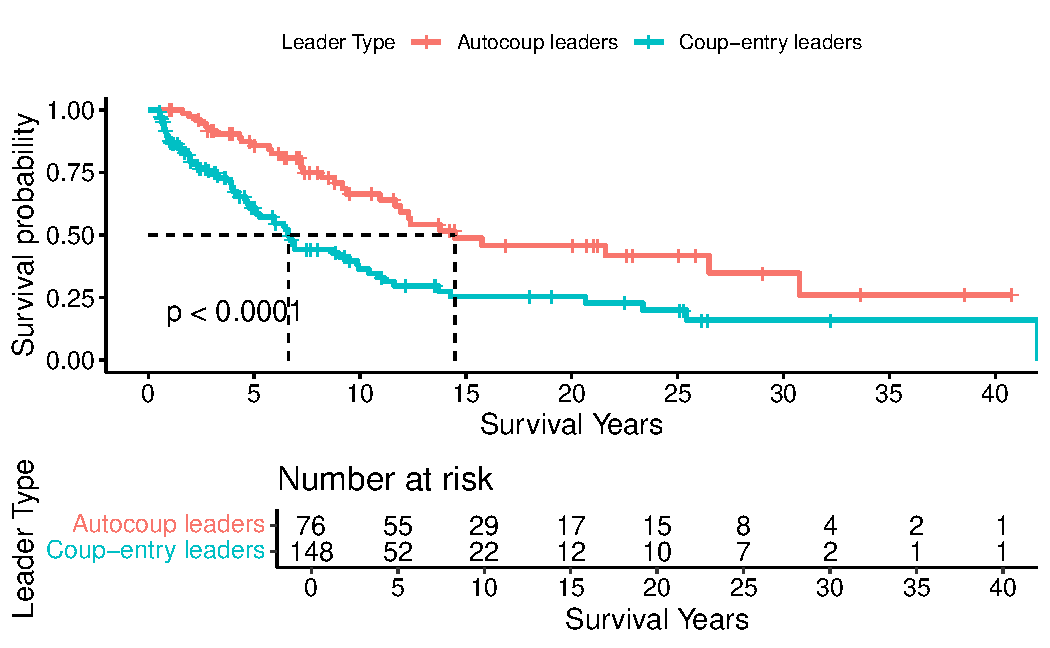
\includegraphics{coups_and_autocoups_files/figure-pdf/fig-logrank-1.pdf}

}

\caption{\label{fig-logrank}Survival curves of overstaying and
coup-entry leaders}

\end{figure}%

A preliminary log-rank test in survival analysis, as illustrated in
Figure~\ref{fig-logrank}, demonstrates a statistically significant
difference between the tenures of autocoup and coup-entry leaders. The
survival curve for autocoup leaders consistently surpasses that of
coup-entry leaders, indicating longer survival tenures and a lower risk
of ouster for autocoup leaders.

I posit that the method of accession significantly influences leadership
longevity. Coup-entry leaders likely face greater challenges to their
rule, resulting in shorter average tenures compared to autocoup leaders.
The analysis, using Cox proportional hazards and time-dependent Cox
models, supports this hypothesis, showing that autocoup leaders
generally experience longer tenures than coup-entry leaders.

This study offers two key contributions to the field. First, it
highlights an understudied factor in leadership survival analysis: the
impact of the method of accession to power. Our findings suggest that
leaders' survival is influenced not only by their ruling strategies
after taking power but also by how they initially acquired it. Second,
by employing survival models, this research provides empirical evidence
of the significant difference in tenure duration between autocoup and
coup-entry leaders. This insight may help explain the increasing
prevalence of power extensions through autocoups since 2000, as more
incumbents observe and potentially emulate successful precedents.

The remainder of this chapter is structured as follows: Section 2
provides a comprehensive literature review on political survival,
establishing the context for this research. Section 3 explores the
factors influencing the survival of coup and autocoup leaders. Section 4
outlines the methodology and data used, including the application of
survival models to analyze the determinants of leadership longevity.
Section 5 presents the findings of the analysis and a detailed
discussion of the results. Finally, Section 6 concludes by synthesizing
the key takeaways and exploring their broader implications for political
stability and democratic processes.

\section{Literature review}\label{literature-review}

Political survival has been a cornerstone of political science research
for decades, driven by the wide-ranging variations observed across
regimes, countries, and historical periods. This field of study
encompasses two crucial and interconnected aspects: regime survival and
individual leader survival.

Regime survival focuses on the longevity of political systems, such as
monarchies, political parties, or specific ideological structures. In
contrast, leader survival concerns the duration of individual leaders'
time in office. These concepts often exhibit contrasting patterns. For
instance, in parliamentary democracies like Japan or the UK, specific
political parties may hold power for extended periods while individual
leaders (Prime Ministers) change frequently. Similarly, communist
regimes typically see long-lasting parties in power, with more frequent
leadership transitions. Presidential systems like the United States or
some military regimes experience more frequent changes in both the
ruling party or junta and the country's leader. This study specifically
investigates the dynamics of individual leader survival, focusing on the
factors influencing how long leaders remain in power.

The existing literature on leader survival is vast and multifaceted.
Some studies explore specific mechanisms influencing leadership
longevity within particular regimes, such as democracies
(\citeproc{ref-svolik2014}{Svolik 2014}) or autocracies
(\citeproc{ref-davenport2021}{Davenport, RezaeeDaryakenari, and Wood
2021}). Others aim to develop more generalizable theoretical frameworks
explaining leader survival across diverse political systems
(\citeproc{ref-buenodemesquita2003}{Bueno de Mesquita et al. 2003}).
While the development of a universal theory remains an alluring goal, it
is important to acknowledge the inherent challenges in creating a single
model that encompasses the complexities of leadership survival across
all regime types.

Power transition mechanisms vary significantly across different regimes,
particularly between democracies and autocracies. In many autocratic
systems, leadership selection is a closed affair, often restricted to a
narrow pool such as royal families, military elites, or ruling party
members. While political competition and elections may exist in some
autocracies, significant barriers to entry for legitimate challengers
often persist. Potential rivals may face threats such as assassination,
imprisonment, or exile. Moreover, selection processes are often shrouded
in secrecy, making it challenging to gauge true levels of public support
compared to democracies. Consequently, calculating selectorates or
winning coalitions, as explored by Bueno de Mesquita et al.
(\citeproc{ref-buenodemesquita2003}{2003}), becomes nearly impossible in
many autocracies.

Given these complexities, focusing research on more specific regimes or
types of leaders may be more appropriate. While regular and anticipated
leadership changes are important, they offer less fertile ground for
exploring the dynamics of leader longevity, as the vast majority of
leaders who assume power through established channels also exit power
through established mechanisms (\citeproc{ref-goemans2009}{Goemans,
Gleditsch, and Chiozza 2009}). In contrast, the study of political
survival among irregular leaders is particularly captivating due to the
intricacies and uncertainties associated with irregular leadership
transitions.

Two primary perspectives have emerged to explain the dynamics of leader
survival:

\begin{itemize}
\item
  \textbf{Objective factors and resources:} This perspective considers
  elements such as personal competence (\citeproc{ref-yu2016}{Yu and
  Jong-A-Pin 2016}), societal stability
  (\citeproc{ref-arriola2009}{Arriola 2009}), economic development
  (\citeproc{ref-palmer1999}{Palmer and Whitten 1999};
  \citeproc{ref-williams2011}{Williams 2011}), access to natural
  resources (\citeproc{ref-smith2004}{Smith 2004};
  \citeproc{ref-quirozflores2012}{Quiroz Flores and Smith 2012};
  \citeproc{ref-wright2013}{Wright, Frantz, and Geddes 2013}), and
  external support networks (\citeproc{ref-licht2009}{Licht 2009};
  \citeproc{ref-wright2008}{Wright 2008}; \citeproc{ref-thyne2017}{C.
  Thyne et al. 2017}).
\item
  \textbf{Subjective factors and strategies:} This approach explores the
  strategies leaders employ to consolidate their power, encompassing
  both the formulation and implementation of political policies and
  leaders' responses to opposition, challenges, or even coups and
  rebellions (\citeproc{ref-gandhi2007}{Gandhi and Przeworski 2007};
  \citeproc{ref-morrison2009}{Morrison 2009};
  \citeproc{ref-escribuxe0-folch2013}{Escribà-Folch 2013};
  \citeproc{ref-davenport2021}{Davenport, RezaeeDaryakenari, and Wood
  2021}).
\end{itemize}

Coups have garnered significant scholarly attention due to their pivotal
role in removing leaders (\citeproc{ref-svolik2009}{Svolik 2009};
\citeproc{ref-frantz2016}{Frantz and Stein 2016}). Existing research
delves into strategies for thwarting coups (\citeproc{ref-powell2017}{J.
Powell 2017}; \citeproc{ref-sudduth2017}{Sudduth 2017};
\citeproc{ref-debruin2020}{De Bruin 2020}) and how leaders extend their
tenures after surviving coup attempts (\citeproc{ref-easton2018}{Easton
and Siverson 2018}). Sudduth (\citeproc{ref-sudduth2017}{2017}) examines
post-coup actions of dictators, focusing on purge strategies, while
Sudduth and Bell (\citeproc{ref-sudduth2018}{2018}) investigates how
leaders' entry methods affect their removal in dictatorships.

Despite the extensive research on leader survival across various
contexts, a significant gap persists. There is a lack of research
specifically exploring and comparing the survival tenures of leaders who
extend their reigns through autocoups compared to coup-entry leaders.
This study aims to address this gap by investigating and comparing the
duration of leadership survival between these two distinct leader types,
contributing to a more nuanced understanding of political survival in
irregular leadership transitions.

\section{Survival dynamics of autocoup and coup-entry
leaders}\label{survival-dynamics-of-autocoup-and-coup-entry-leaders}

\subsection{Autocoup leaders versus coup-entry
leaders}\label{autocoup-leaders-versus-coup-entry-leaders}

As highlighted in the previous section, investigating leadership
survival presents inherent challenges due to factors such as the opacity
and diverse mechanisms of power transitions. However, these challenges
underscore the significance of this research, as it illuminates
understudied dynamics in political leadership.

While the survival of political leaders exhibits complexity and
variation, it is not entirely devoid of patterns. Leaders of similar
types often display significant comparability. Before delving into this
comparison, it is essential to clarify several key terminologies.

Firstly, the concepts of coup and autocoup adhere to the definitions
established in Section~\ref{sec-chapter2} and Section~\ref{sec-chapter3}
respectively. However, a significant disparity exists in the tenure
lengths of coup-entry leaders and autocoup leaders. Many coup-entry
leaders rule for only a few months or even days, while autocoup leaders
typically enjoy longer tenures after their power grab. To ensure
meaningful analysis, this chpater focuses on leaders with more
substantial periods in power. As defined in Section~\ref{sec-chapter3},
an autocoup is considered successful if the power extension lasts for at
least six months. For consistency and to allow for more robust
comparison, this chapter applies the same six-month threshold to both
autocoup and coup-entry leaders. This approach differs from the
seven-day duration used by J. M. Powell and Thyne
(\citeproc{ref-powell2011}{2011}) for traditional coups, allowing us to
examine more established leadership periods and their associated
dynamics.

Secondly, it is crucial to distinguish between an autocoup leader and a
coup-entry leader, as leadership survival is the primary focus of this
study:

\begin{itemize}
\item
  \textbf{Autocoup leader:} This refers to an incumbent leader who
  successfully uses illegitimate or unconstitutional means to extend
  their tenure in power. In an autocoup, the leader orchestrates the
  power grab and continues to rule afterwards.
\item
  \textbf{Coup-entry leader:} This term designates the individual who
  assumes power after a successful coup. The coup leader and the
  coup-entry leader may or may not be the same person. Unlike autocoups,
  coups often involve multiple leaders (individuals or groups) who
  overthrow the incumbent leader, but typically only one of them assumes
  supreme power. In some instances, coup leaders may support someone
  outside the coup plot to become the new leader, such as military
  officers returning power to civilians or supporting a new general
  election. Regardless of the specific scenario, a coup-entry leader in
  this study refers to the individual who assumes formal leadership
  following a successful coup.
\end{itemize}

Given that autocoup leaders typically exhibit longer overall tenures
compared to coup-entry leaders, this study focuses on a more nuanced
comparison. Specifically, we will analyse the \textbf{post-autocoup}
tenure of autocoup leaders and contrast it with the \textbf{post-coup}
tenure of coup-entry leaders. This examination is motivated by the
relevance and similarity of these leader types in terms of illegitimacy,
uncertainty, and instability.

\subsection{Different challenges and tactics to consolidate
power}\label{different-challenges-and-tactics-to-consolidate-power}

Previous research has established that the ability to skillfully retain
power is the primary determinant of leader longevity. Leaders who can
maintain control or manipulate the balance of power tend to have longer
tenures. However, coup-entry and autocoup leaders face distinct
challenges in consolidating their power, primarily due to differences in
the intensity of issues related to illegitimacy, uncertainty, and
instability. This disparity creates an uneven playing field in terms of
power dynamics, with coup-entry leaders at a significant disadvantage.
The following analysis examines these challenges and their impact on
leader tenure.

\subsubsection{Illegitimacy: Both coup-entry and autocoup leaders suffer
from a legitimacy deficit, but the nature of this deficit
differs}\label{illegitimacy-both-coup-entry-and-autocoup-leaders-suffer-from-a-legitimacy-deficit-but-the-nature-of-this-deficit-differs}

While both coup-entry and autocoup leaders suffer from a legitimacy
deficit, the nature of this deficit differs. Coup leaders openly seize
power, making their illegitimacy explicit. Conversely, autocoup leaders
employ a deceptive strategy, manipulating legal processes to create a
facade of democratic legitimacy. Despite this veneer, their actions
fundamentally undermine democratic principles. Scholars have suggested
alternative terms like ``incumbent overstay'' or ``executive takeover''
to reflect the less overt nature of power grabs in these cases. This
perceived legitimacy can provide autocoup leaders with a temporary
advantage as opponents are often restricted to legal challenges.

\subsubsection{\texorpdfstring{\textbf{Uncertainty:} The irregular paths
to power taken by both types of leaders create uncertainty regarding
their reigns and eventual
departures}{Uncertainty: The irregular paths to power taken by both types of leaders create uncertainty regarding their reigns and eventual departures}}\label{uncertainty-the-irregular-paths-to-power-taken-by-both-types-of-leaders-create-uncertainty-regarding-their-reigns-and-eventual-departures}

The irregular paths to power taken by coup-initiators and autocoup
leaders create uncertainty regarding their reigns and eventual
departures. Their ascension through irregular means undermines
established power transition norms, leaving doubts about their
commitment to constitutional succession protocols. This uncertainty not
only unsettles elites and citizens but also plagues the leaders
themselves, who grapple with the ambiguity surrounding the transfer of
power -- when, how, and to whom. Historical analyses underscore this
predicament, with data revealing that more than two-thirds of irregular
exits from leadership stem from coup-related upheavals
(\citeproc{ref-goemans2009}{Goemans, Gleditsch, and Chiozza 2009}).

Coup-entry and autocoup leaders face different levels of uncertainty
following their rise to power. After a coup, three major uncertainties
arise:

\begin{itemize}
\item
  \textbf{Leadership Assumption}: It is unclear who will assume
  leadership. Although coup leaders often take power, some may return or
  promise to return power to civilian leaders. Even among coup leaders,
  determining who will lead can be problematic, as coup plotters are
  sometimes a group without a clear core leader. For instance, following
  the 1973 Chilean coup, the initial plan for a rotating presidency
  among military leaders was abandoned when General Pinochet
  consolidated control and remained in power until 1990
  (\citeproc{ref-svolik2014}{Svolik 2014}).
\item
  \textbf{Duration of Rule}: The duration of the coup leader's rule is
  uncertain. Leaders like Gamal Abdel Nasser in Egypt (1954 coup),
  Muammar Gaddafi in Libya (1969 coup), and Idi Amin in Uganda (1971
  coup) aimed to retain power for life
  (\citeproc{ref-geddes2018}{Geddes, Wright, and Frantz 2018}), but
  their ability to do so was uncertain. Others promise to transfer power
  to civilian authorities, but the timing and fulfilment of these
  promises are unclear. For example, Myanmar's military junta (2021
  coup) has repeatedly extended a state of emergency, clinging to power
  beyond the promised time-frame\footnote{https://thediplomat.com/2023/08/myanmar-junta-extends-state-of-emergency-for-fourth-time/:
    Myanmar\\
    Junta Extends State of Emergency for Fourth Time. Accessed on
    2024-08-05.}. Conversely, after the 2010 coup in Niger, the military
  honoured their promise by restoring civilian rule within the same year
  (\citeproc{ref-ginsburg2019}{Ginsburg and Elkins 2019}).
\item
  \textbf{Succession}: The successors of coup leaders are uncertain.
  Some may designate successors from their inner circle, including
  family members, while others may support general elections, though
  whether this will be fulfilled as intended remains uncertain.
\end{itemize}

In contrast, autocoup leaders present a clearer picture regarding
leadership and tenure. There is no ambiguity about who will rule after
an autocoup. In the medium term, autocoup leaders typically hold office
themselves. Many, like Putin in Russia and Xi Jinping in China, seek to
extend their rule indefinitely and are unlikely to relinquish power
voluntarily. Others attempt to extend their terms incrementally, such as
President Menem of Argentina, who overstayed successfully in 1993 but
failed in his bid for another term in 1999
(\citeproc{ref-llanos2019}{Llanos 2019}).

\subsubsection{\texorpdfstring{\textbf{Instability:} The awareness of
shaky legitimacy and persistent uncertainty breeds insecurity and a
sense of
crisis}{Instability: The awareness of shaky legitimacy and persistent uncertainty breeds insecurity and a sense of crisis}}\label{instability-the-awareness-of-shaky-legitimacy-and-persistent-uncertainty-breeds-insecurity-and-a-sense-of-crisis}

The awareness of their shaky legitimacy and the persistent uncertainty
breeds insecurity and a perpetual sense of crisis among coup-entry and
autocoup leaders. In a bid to solidify their grip on power, they often
resort to reshaping power dynamics or purging potential adversaries.
Paradoxically, these attempts to bolster stability frequently backfire,
unleashing greater turmoil and instability.

The stability of a regime, particularly in an autocracy, hinges on
maintaining a balance of power. Coups, however, inevitably disrupt this
balance, even when they are bloodless, necessitating the creation of a
new equilibrium. The ousting of previous rulers requires dismantling the
established governing structure and reshuffling high-ranking officials,
actions that inherently generate instability and create adversaries for
the new leadership. This makes restoring order and establishing a
balanced power structure notably challenging. Studies show that new
leaders often purge rival elite groups to consolidate their power at the
outset of their tenure (\citeproc{ref-sudduth2017}{Sudduth 2017};
\citeproc{ref-roessler2011}{Roessler 2011}).

Such actions can provoke backlash even from close allies. For instance,
in Uganda, President Obote's attempt to undermine the army
commander-in-chief, Idi Amin, led to Amin gaining the army's support and
ultimately ousting Obote in a 1971 coup. Similarly, in Pakistan in 1999,
shortly after Prime Minister Sharif dismissed powerful army chief
General Pervez Musharraf, Sharif himself was ousted in a coup
orchestrated by Musharraf and his supporters
(\citeproc{ref-sudduth2017}{Sudduth 2017}).

To consolidate power, coup-entry leaders often have to compromise with
internal or external power challengers. However, these compromises are
frequently unstable and easily broken. The situation becomes even more
complex when there is a risk of civil war. Leaders may attempt to reduce
the likelihood of subsequent coups, potentially increasing the chances
of societal rebellions and civil wars
(\citeproc{ref-roessler2011}{Roessler 2011}).

Moreover, instability extends beyond leadership to policies. A new
leadership group often brings new policies, and coups are sometimes
triggered by disagreements over significant policies. Major policy
shifts can instigate dissent or grievances from various ruling factions,
communities, regions, ethnicities, or religions. In contrast, autocoup
leaders encounter fewer of these issues, as their regimes experience
fewer abrupt changes. They face less pressure to dismantle the existing
ruling paradigm and establish a new order. Even when adjustments are
necessary, they have more time to implement changes gradually.

\begingroup
\setlength\LTleft{0\linewidth}
\setlength\LTright{0\linewidth}\fontsize{12.0pt}{14.4pt}\selectfont

\begin{longtable}{@{\extracolsep{\fill}}>{\raggedright\arraybackslash}p{\dimexpr 75.00pt -2\tabcolsep-1.5\arrayrulewidth}>{\raggedright\arraybackslash}p{\dimexpr 187.50pt -2\tabcolsep-1.5\arrayrulewidth}>{\raggedright\arraybackslash}p{\dimexpr 187.50pt -2\tabcolsep-1.5\arrayrulewidth}}

\caption{\label{tbl-leaders}Main features of autocoup and coup-entry
leaders}

\tabularnewline

\toprule
Feature & Autocoup Leader & Coup Entry Leader \\ 
\midrule\addlinespace[2.5pt]
Illegitimacy & Normally attained through
lawful procedures, but
lacking consensus
legitimacy & Blatantly illegal \\ 
{\cellcolor[HTML]{EDEDE9}{\textcolor[HTML]{000000}{Uncertainty}}} & {\cellcolor[HTML]{EDEDE9}{\textcolor[HTML]{000000}{Initially with some certainty, but decreases as the leader's age grows or health worsens}}} & {\cellcolor[HTML]{EDEDE9}{\textcolor[HTML]{000000}{Significant uncertainty initially}}} \\ 
Instability & Relatively stable & Unstable except when a strongman emerges or constitutional institutions are established \\ 
{\cellcolor[HTML]{EDEDE9}{\textcolor[HTML]{000000}{Balance of Power}}} & {\cellcolor[HTML]{EDEDE9}{\textcolor[HTML]{000000}{Generally in a better position of power}}} & {\cellcolor[HTML]{EDEDE9}{\textcolor[HTML]{000000}{Initially unclear and challenging to establish a balance}}} \\ 
\bottomrule

\end{longtable}

\endgroup

Coup-entry leaders face significantly greater challenges in
consolidating power compared to autocoup leaders. This disadvantage
creates a self-perpetuating cycle. Weaker leaders struggle to attract
and retain strong support, making them more vulnerable to internal and
external challenges. The perception of risk discourages potential
allies, further eroding their power base.

Empirical evidence supports this dynamic. Data reveals a correlation
between the frequency of coup attempts in a country and the likelihood
of future coups. For example, Table~\ref{tbl-coups} shows over a third
of coups occurring in the top ten countries with the most attempts since
1950. This suggests that the more coups occur in a country, the more
likely additional coups are to happen in the future.

Conversely, autocoup leaders, often benefiting from a veneer of
legitimacy and a stronger initial position, are better able to
consolidate power and attract supporters. This advantage can be
self-reinforcing, as a strong power base discourages challenges and
fosters loyalty. This dynamic is evident in cases like China (2018),
where the National People's Congress granted Xi Jinping the potential to
rule for life\footnote{https://www.bbc.co.uk/news/world-asia-china-43361276:
  China's Xi allowed to remain `president for life' as\\
  term limits removed. Accessed on 2024-08-05.}, and Russia (2020),
where constitutional changes allow Putin to potentially remain in power
until 2036\footnote{https://www.ucl.ac.uk/news/2020/jul/analysis-vladimir-putin-secures-constitutional-changes-allowing-him-rule-until-2036:
  Analysis: Vladimir Putin secures constitutional changes allowing him
  to rule until 2036. Accessed on 2024-08-05.}.

These factors contribute to a shorter expected tenure for coup-entry
leaders compared to the relatively longer tenures of autocoup leaders.
The average survival period following an autocoup is approximately five
years longer than that of coup-entry leaders (Figure~\ref{fig-logrank}).
Based on these observations, I propose the following hypothesis:

\begin{quote}
\textbf{\emph{H1: Political leaders who successfully extend their tenure
through autocoups are more likely to survive longer compared to
coup-entry leaders.}}
\end{quote}

\section{Research Design}\label{research-design-1}

\subsection{Methodology: Survival
analysis}\label{methodology-survival-analysis}

To test the hypothesis, I will employ two Cox models to analyze the
survival tenures of coup-entry leaders and autocoup leaders. Unlike the
Kaplan-Meier model, the Cox model allows for the estimation of the
impacts of multiple factors. Although it does not directly estimate the
duration of tenure in office, it evaluates the hazard rate associated
with being ousted from power. Essentially, this represents different
facets of the same phenomenon: as a leader's cumulative hazard of being
ousted increases, their probability of survival in office decreases.

The first model will utilize the Cox proportional hazards model (Cox PH
model), using only the variables present at the entry year, without
considering changes in these variables over the leaders' survival times.

However, apart from the primary variable of interest in this
research---the leader type---control variables such as economic
performance, Polity5 scores, and political stability do change over
time. Therefore, the second model will account for these variations by
using the time-dependent Cox model.

\subsection{Dependent variables}\label{dependent-variables}

\begin{itemize}
\item
  \textbf{Survival Time:} The duration of a leader's tenure, measured in
  days. For coup-entry leaders, the survival time begins on the day they
  assume power through a coup. For autocoup leaders, the survival time
  starts on the expiration date of their original legitimate term. For
  example, Xi Jinping assumed power in 2013 and removed term limits in
  2018. His original legitimate tenure was set to end in 2023, so his
  survival time begins in 2023, marking the start of his post-autocoup
  tenure. The survival time concludes on the day the leader exits
  office, applicable to both coup-entry and autocoup leaders.
\item
  \textbf{End point status:} This variable indicates the manner in which
  the leader's tenure concluded, categorized as follows:

  \begin{itemize}
  \item
    \textbf{0 = Censored:} This status is assigned to leaders who leave
    office through regular means other than being ousted. This includes
    leaders transferring power to their designated successors, leaving
    office as their terms expire, losing in general elections,
    voluntarily leaving office due to health issues, or dying of natural
    causes.
  \item
    \textbf{1 = Ousted:} This status is assigned to leaders who are
    forced to leave office. This includes leaders resigning under
    pressure, being ousted by coups or other forces, or being
    assassinated.
  \end{itemize}
\end{itemize}

\subsection{Key Independent variable: Leader
type}\label{key-independent-variable-leader-type}

This variable categorizes leaders into two distinct groups:

\begin{itemize}
\tightlist
\item
  \textbf{Group A = Autocoup Leader}: Leaders who extend their tenure
  through autocoups.
\item
  \textbf{Group B = Coup-Entry Leader}: Leaders who assume power through
  coups.
\end{itemize}

This variable is the primary independent variable of interest, serving
as the basis for comparing the survival time between these two types of
leaders.

The data for both dependent and independent variables are sourced from
the autocoup dataset introduced in this study, Archigos, and PLAD.

\subsection{Control variables}\label{control-variables-1}

\begin{itemize}
\item
  \textbf{Economic Performance:} This variable is measured using two
  indicators: economic level and economic growth trend.

  \begin{itemize}
  \item
    \textbf{Economic Level:} Represented by GDP per capita. This measure
    provides an indication of the overall economic health and standard
    of living in a country.
  \item
    \textbf{Economic Growth Trend:} Assessed using the current-trend
    ratio, developed by Krishnarajan
    (\citeproc{ref-krishnarajan2019}{2019}), which is consistent with
    Equation~\ref{eq-eq6} in chapters 2 and 3.
  \end{itemize}
\end{itemize}

The GDP per capita data, expressed in constant 2017 international
dollars (PPP) and measured in units of \$10,000, is sourced from the
V-Dem dataset by Fariss et al. (\citeproc{ref-fariss2022}{2022}). To
account for the economic impact of the previous year, this data is
lagged by one year.

\begin{itemize}
\item
  \textbf{Political Stability:} This variable captures overall regime
  stability by including a violence index that encompasses all types of
  internal and interstate wars and violence. The data for this index is
  sourced from the Major Episodes of Political Violence dataset by
  Marshall (\citeproc{ref-marshall2005current}{2005}). This index
  provides a comprehensive measure of the level of violence and conflict
  within a country, which can significantly impact leadership survival.
\item
  \textbf{Degree of Democracy:} The level of democracy is gauged using
  Polity 5 scores at the entry year for each respective country. These
  scores range from -10 (fully autocratic) to +10 (fully democratic),
  capturing the extent of democratic versus autocratic governance. This
  dataset is sourced from the Center for Systemic Peace (CSP) and
  provides an essential measure of political regime type, which can
  influence the stability and survival of leaders in power.
\item
  \textbf{Population Size:} To account for its potential impact on
  leaders' tenures, the log of the population size is considered. This
  transformation helps in managing the wide range of population sizes
  across different countries. The data is sourced from the V-Dem dataset
  and is evaluated to understand its influence on leadership survival.
  Larger populations may present more governance challenges and
  potential sources of opposition, thereby affecting the stability and
  longevity of a leader's tenure.
\item
  \textbf{Leader's Age:} The age of the leader at the entry year is
  included as an additional variable in the analysis, offering insights
  into potential correlations with leadership survival. Older leaders
  may have different experiences, networks, and health considerations
  that could influence their ability to maintain power. This data is
  sourced from the leaders dataset by Archigos and PLAD.
\end{itemize}

\section{Results and discussion}\label{results-and-discussion-1}

\subsection{Model results}\label{model-results}

Using the \texttt{survival} package in R
(\citeproc{ref-survival}{Therneau 2024}), I present the regression
results for both the Cox Proportional Hazards (Cox PH) model and the
time-dependent Cox model in Table~\ref{tbl-cox}.

\begingroup
\fontsize{12.0pt}{14.4pt}\selectfont
\setlength{\LTpost}{0mm}

\begin{longtable}{lcccccccc}

\caption{\label{tbl-cox}Cox models for survival time of different types
of leaders}

\tabularnewline

\toprule
 & \multicolumn{4}{c}{\textbf{Cox PH Model}} & \multicolumn{4}{c}{\textbf{Time-dependent Cox Model}} \\ 
\cmidrule(lr){2-5} \cmidrule(lr){6-9}
\textbf{Characteristic} & \textbf{N} & \textbf{Event N} & \textbf{HR}\textsuperscript{\textit{1,2}} & \textbf{SE}\textsuperscript{\textit{2}} & \textbf{N} & \textbf{Event N} & \textbf{HR}\textsuperscript{\textit{1,2}} & \textbf{SE}\textsuperscript{\textit{2}} \\ 
\midrule\addlinespace[2.5pt]
{\bfseries Leader Type} &  &  &  &  &  &  &  &  \\ 
    Autocoup leaders & 76 & 31 & 1.00 & — & 737 & 29 & 1.00 & — \\ 
    Coup-entry leaders & 148 & 73 & 2.71*** & 0.252 & 853 & 73 & 2.23*** & 0.246 \\ 
{\bfseries GDP Growth Trend} & 224 & 104 & 1.95 & 1.08 & 1,590 & 102 & 0.20* & 0.981 \\ 
{\bfseries GDP per capita} & 224 & 104 & 0.97* & 0.020 & 1,590 & 102 & 0.95** & 0.023 \\ 
{\bfseries Population: log} & 224 & 104 & 0.98 & 0.083 & 1,590 & 102 & 0.90 & 0.079 \\ 
{\bfseries Polity 5} & 224 & 104 & 0.99 & 0.025 & 1,590 & 102 & 1.01 & 0.023 \\ 
{\bfseries Political stability} & 224 & 104 & 1.00 & 0.053 & 1,590 & 102 & 1.11* & 0.049 \\ 
{\bfseries Age} & 224 & 104 & 1.01 & 0.010 & 1,590 & 102 & 1.00 & 0.011 \\ 
\bottomrule

\end{longtable}

\begin{minipage}{\linewidth}
\textsuperscript{\textit{1}}*p\textless{}0.1; **p\textless{}0.05; ***p\textless{}0.01\\
\textsuperscript{\textit{2}}HR = Hazard Ratio, SE = Standard Error\\
\end{minipage}
\endgroup

Both the Cox PH model and the time-dependent Cox model analyses revealed
a statistically significant association between leadership type and the
hazard of removal from power. Since time-dependent Cox model use the
control variables which change over time, I interpret the main findings
based on time-dependent model.

Coup-entry leaders were found to have a hazard ratio of 2.23 in the
time-dependent model compared to autocoup leaders (reference group),
assuming all other variables in the model are held constant. This
suggests that coup-entry leaders face a significantly greater risk of
removal from power compared to autocoup leaders. At any given time
during their tenure, coup-entry leaders are 2.23 times more likely to be
ousted from power compared to autocoup leaders, all else being equal in
the model.

The control variables perform differently in the two models. Economic
level (GDP per capita) exhibits statistically significant effects in
both models. In the time-dependent model, the hazard ratio of 0.95
indicates that for each unit increase in GDP per capita (measured in
units of \$10,000), the hazard (or risk) of being ousted at any given
time is reduced by 5\%, assuming all other variables in the model are
held constant.

GDP growth trend demonstrates a more substantial effect in reducing the
risk of coups. Specifically, a 1 percentage point higher economic growth
trend is associated with an 80\% reduction in the risk of being ousted,
although this effect is only statistically significant at the 10\%
level. This suggests a possible trend where positive economic
performance might mitigate the risk of removal from power, but the
evidence is not robust enough to confirm this conclusively.

Political stability, as measured by the violence index, shows that a
1-point increase in the index correlates with an 11\% higher risk of
being ousted. However, this effect is also only statistically
significant at the 10\% level, indicating a weaker but potentially
important relationship between increased violence and the risk of
removal from office.

\subsection{Discussion}\label{discussion}

\begin{figure}

\begin{minipage}{0.50\linewidth}

\centering{

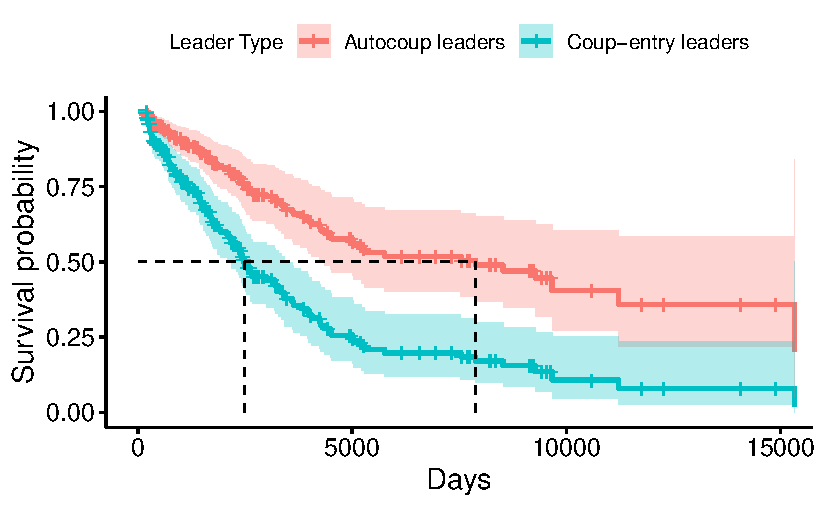
\includegraphics{coups_and_autocoups_files/figure-pdf/fig-coxSurv-1.pdf}

}

\subcaption{\label{fig-coxSurv-1}Cox PH Model}

\end{minipage}%
%
\begin{minipage}{0.50\linewidth}

\centering{

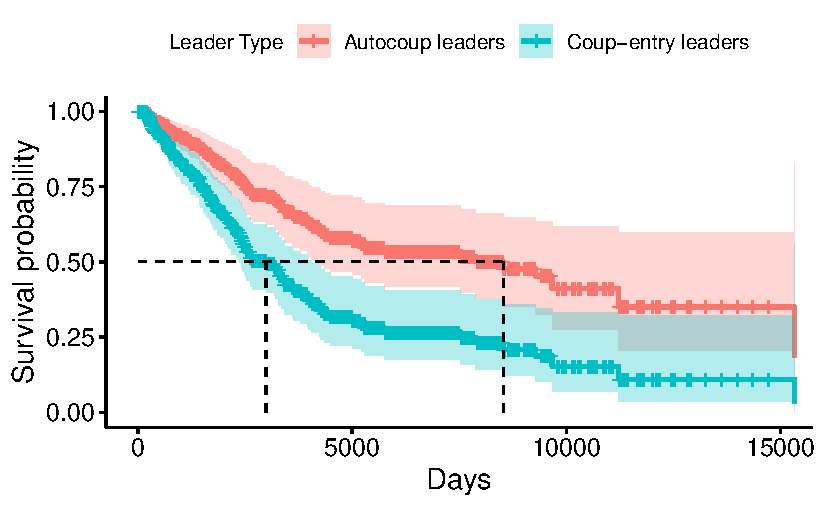
\includegraphics{coups_and_autocoups_files/figure-pdf/fig-coxSurv-2.pdf}

}

\subcaption{\label{fig-coxSurv-2}Time-dependent Cox Model}

\end{minipage}%

\caption{\label{fig-coxSurv}Survival curves for Cox Model}

\end{figure}%

The survival curves depicted in Figure~\ref{fig-coxSurv} illustrate the
survival rates for leaders of both types. Both the Cox PH model and the
time-dependent Cox model produce similar plots. Notably, the survival
curve for coup-entry leaders exhibits a significantly lower trajectory
compared to that of autocoup leaders. The steeper drop at the early
stage for coup-entry leaders indicates they are more likely to be ousted
shortly after assuming power. Additionally, the survival curve for
coup-entry leaders crosses the median survival line much earlier (about
3,000 days) than that of autocoup leaders (about 8,500 days). This
disparity suggests that autocoup leaders tend to remain in power for
longer durations than their coup-entry counterparts.

\begin{figure}

\begin{minipage}{0.50\linewidth}

\begin{verbatim}
Call:
coxph(formula = Surv(T1, T2, status) ~ group + GDP_trend + GDP_pc + 
    pop_log + polity5 + violence + age, data = Mydata2, cluster = id)

  n= 1590, number of events= 102 

                             coef exp(coef)  se(coef) robust se      z Pr(>|z|)
groupCoup-entry leaders  0.802158  2.230348  0.245712  0.243824  3.290   0.0010
GDP_trend               -1.589431  0.204042  0.981002  0.911011 -1.745   0.0810
GDP_pc                  -0.046171  0.954878  0.022800  0.018675 -2.472   0.0134
pop_log                 -0.101345  0.903621  0.078758  0.078379 -1.293   0.1960
polity5                  0.006888  1.006912  0.022551  0.023234  0.296   0.7669
violence                 0.101338  1.106651  0.048960  0.052556  1.928   0.0538
age                      0.004961  1.004973  0.010516  0.010734  0.462   0.6440
                          
groupCoup-entry leaders **
GDP_trend               . 
GDP_pc                  * 
pop_log                   
polity5                   
violence                . 
age                       
---
Signif. codes:  0 '***' 0.001 '**' 0.01 '*' 0.05 '.' 0.1 ' ' 1

                        exp(coef) exp(-coef) lower .95 upper .95
groupCoup-entry leaders    2.2303     0.4484   1.38302    3.5968
GDP_trend                  0.2040     4.9010   0.03422    1.2167
GDP_pc                     0.9549     1.0473   0.92056    0.9905
pop_log                    0.9036     1.1067   0.77494    1.0537
polity5                    1.0069     0.9931   0.96209    1.0538
violence                   1.1067     0.9036   0.99833    1.2267
age                        1.0050     0.9951   0.98405    1.0263

Concordance= 0.67  (se = 0.029 )
Likelihood ratio test= 31.77  on 7 df,   p=4e-05
Wald test            = 27.21  on 7 df,   p=3e-04
Score (logrank) test = 28.15  on 7 df,   p=2e-04,   Robust = 27.58  p=3e-04

  (Note: the likelihood ratio and score tests assume independence of
     observations within a cluster, the Wald and robust score tests do not).
\end{verbatim}

\end{minipage}%
%
\begin{minipage}{0.50\linewidth}

\centering{

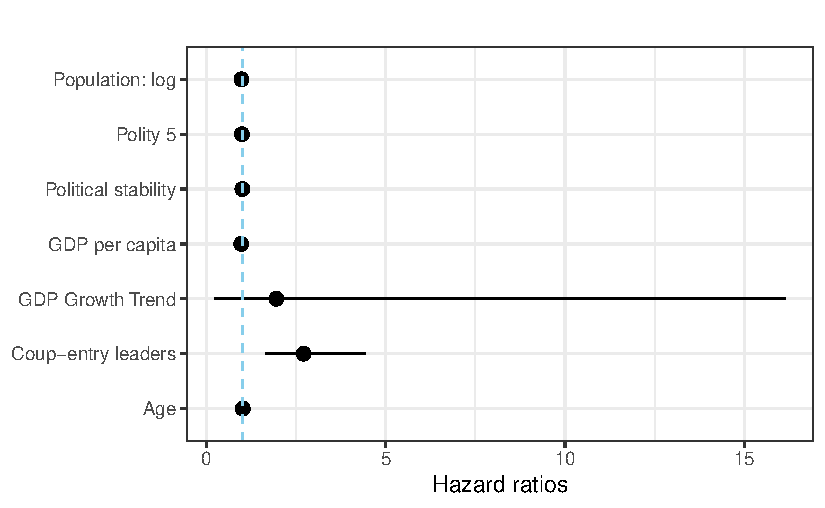
\includegraphics{coups_and_autocoups_files/figure-pdf/fig-coxHR-1.pdf}

}

\subcaption{\label{fig-coxHR-1}Cox PH Model}

\end{minipage}%
\newline
\begin{minipage}{0.50\linewidth}

\centering{

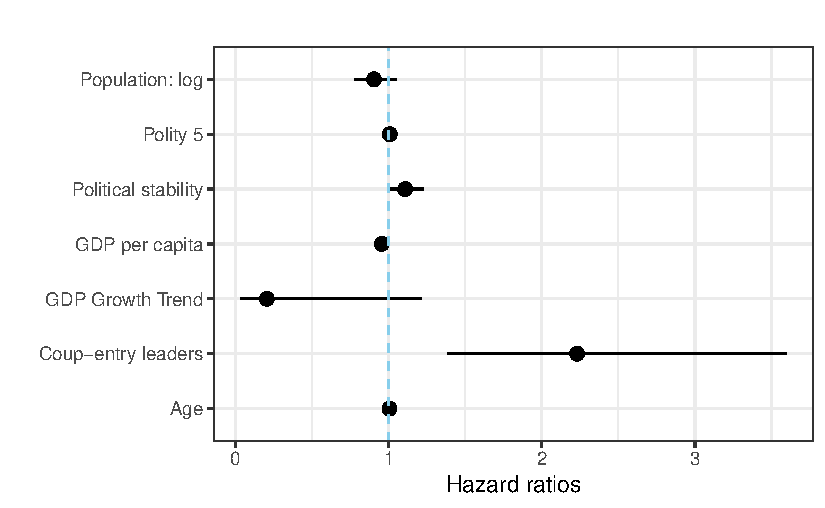
\includegraphics{coups_and_autocoups_files/figure-pdf/fig-coxHR-2.pdf}

}

\subcaption{\label{fig-coxHR-2}Time-dependent Cox Model}

\end{minipage}%

\caption{\label{fig-coxHR}Hazard ratios and 95\% CIs for Leader Ousting}

\end{figure}%

Figure~\ref{fig-coxHR} displays the hazard ratios and corresponding 95\%
confidence intervals for the variables incorporated in the Cox model.
Both the Cox Proportional Hazards (PH) model and the time-dependent
model produce similar plots, reinforcing the robustness of the findings.
Key points to note include:

\begin{itemize}
\item
  The closer the hazard ratio (represented by the dots) is to 1, the
  less impact the variable has on the risk of being ousted. A hazard
  ratio of 1 indicates no effect.
\item
  The whiskers extending from the dots represent the 95\% confidence
  intervals. If these whiskers cross the vertical blue line at 1, it
  indicates that the variable is not statistically significant at the
  5\% level.
\end{itemize}

\begin{itemize}
\item
  The hazard ratio for coup-entry leaders is significantly greater than
  1 and statistically significant at the 5\% level. This indicates that
  coup-entry leaders face a substantially higher risk of being ousted
  compared to autocoup leaders.
\item
  Most other variables have hazard ratios close to 1, suggesting that a
  one-unit increase in these variables does not significantly affect the
  risk of being ousted.
\end{itemize}

\begin{itemize}
\tightlist
\item
  Although the hazard ratio for GDP growth trend is considerably less
  than 1 in the time-dependent model, indicating a potential protective
  effect, it is not statistically significant at the 5\% level. However,
  it is statistically significant at the 10\% level, suggesting that
  better economic performance may help to consolidate the rule of the
  incumbents to some extent, albeit the evidence is not as strong.
\end{itemize}

\subsection{Assessing the Proportional Hazards
Assumption}\label{assessing-the-proportional-hazards-assumption}

Assessing the proportional hazards assumption is crucial for the
validity of the Cox model results. To evaluate this, we used the
chi-square test based on Schoenfeld residuals to determine whether the
covariate effects remain constant (proportional) over time. Although the
Cox PH model violates the proportional hazards assumption, our primary
analysis relies on the time-dependent Cox model, which does not show
strong evidence of violating the proportional hazards assumption for any
covariate. The global p-value of 0.416 is much greater than the 5\%
significance level, indicating that the proportional hazards assumption
is reasonably met for the time-dependent Cox model.

\section{Conclusion}\label{conclusion-2}

This chapter examined the survival durations of political leaders who
come to power through irregular means, specifically coups and autocoups.
I hypothesized that the mode of accession significantly influences
leader tenure. Employing survival analysis techniques, including the Cox
proportional hazards model and a time-dependent Cox model, I found
strong evidence that autocoup leaders generally enjoy longer tenures
than coup-entry leaders.

The findings revealed a significant difference in average tenure, with
post-autocoup leaders averaging approximately 11 years in power compared
to 5.6 years for coup-entry leaders. The time-dependent Cox model
further indicated that coup-entry leaders are 2.23imes more likely to be
ousted from power at any given time compared to autocoup leaders, all
else being equal.

These results highlight the importance of understanding the phenomenon
of autocoups, where leaders extend their rule by manipulating legal
frameworks. Due to the relative ease and potential benefits of
autocoups, this method of power retention might incentivize more leaders
to employ it. Consequently, democratic backsliding could become more
prevalent as autocoups weaken democratic institutions and constitutional
norms, particularly in nascent democracies or those transitioning from
autocracy.

This study contributes to the field of leadership survival by
demonstrating that the mode of accession significantly impacts leader
tenure, a factor previously under-explored in the literature. By
utilizing both Cox models, the research offers robust analytical
techniques for studying political leadership survival and provides
strong evidence of divergent tenure lengths between these two types of
irregular-entry leaders.

However, limitations exist. The study relies heavily on the autocoup
dataset collected and coded by the author. The concept and data itself
are relatively novel within academia. Future research should refine and
establish wider recognition for the term ``autocoup,'' leading to more
accurate and comprehensive data collection efforts. Expanding the
dataset to include more cases and integrating it with data on other
irregular leadership transitions could yield a more holistic
understanding of political survival in such contexts.

Overall, this chapter underscores the need for more nuanced approaches
to studying political tenure and the mechanisms of irregular power
retention, contributing valuable insights into the dynamics of political
stability and the risks associated with different forms of
non-democratic leadership succession.

\chapter{Conclusion}\label{conclusion-3}

\section{Main Findings}\label{main-findings}

This study delves into the dynamics and implications of irregular power
transitions, focusing on coups and autocoups. The findings illuminate
the complex interplay between incumbents and challengers fighting for
power.

Firstly, our analysis reveals that the expected success rate of a coup
attempt significantly influences its likelihood. This success rate is
heavily influenced by the balance of power between the incumbent regime
and challengers, which is largely determined by regime type. We find
that military regimes, although with more control over their own
military forces, face a higher risk of coups compared to dominant-party
regimes.

Secondly, the study introduces a redefined concept: the autocoup.
Defined as an incumbent leader's refusal to relinquish power as
mandated, this research distinguishes autocoups from broader terms like
self-coups. Based on this definition, we present the first publicly
available dataset of autocoup events from 1945 to 2022, encompassing 110
attempts and 87 successful autocoups. Case studies and empirical
analyses demonstrate the dataset's utility for quantitative research,
providing a robust foundation for further analysis on autocoups.

Thirdly, employing survival analysis techniques, the study finds clear
differences in leader longevity between those who come to power through
coups and those who extend their rule through autocoups. The results
indicate that coup-installed leaders face a significantly higher risk of
removal compared to autocoup leaders who manipulate the system to extend
their rule.

\section{Limitations and directions for future
research}\label{limitations-and-directions-for-future-research}

This study offers a novel framework for analysing irregular power
transitions, but some limitations require further exploration:

\begin{itemize}
\item
  \textbf{Data refinement:} Defining and classifying autocoups is a new
  approach. Future research should validate this classification system
  through additional studies and expert evaluations.
\item
  \textbf{Data harmonization:} The current analysis faces challenges due
  to mismatched units (country-year vs.~leader) between coup and
  autocoup datasets. Future efforts should explore data harmonization
  techniques for more robust comparisons.
\item
  \textbf{Democratic backsliding:} While this study establishes a
  connection between irregular power transitions and democratic
  backsliding, further empirical evidence is needed to solidify this
  link.
\end{itemize}

Several avenues exist for future research:

\begin{itemize}
\item
  \textbf{Terminology and data collection:} Refining the ``autocoup''
  concept and achieving wider recognition will facilitate more accurate
  and comprehensive data collection.
\item
  \textbf{Dataset expansion:} Expanding the autocoup dataset with more
  cases and integrating it with data on other irregular leadership
  transitions can provide a more holistic view of political survival
  after these events.
\item
  \textbf{Power dynamics and long-term impacts:} Utilizing this dataset,
  future studies can delve deeper into power dynamics at play and
  explore the long-term consequences of irregular transitions on
  political systems, particularly regarding democratic backsliding,
  breakdown, and personalization of power.
\end{itemize}

In conclusion, this study sheds light on the dynamics of irregular power
transitions, specifically focusing on coups and autocoups. By redefining
autocoups, classifying the dataset, analysing determinants, and
comparing leader longevity, we establish a framework for understanding
irregular transitions and leader survival. This work contributes to a
deeper understanding of democratic resilience and political stability.
Future research can build upon this foundation by conducting further
empirical analyses based on the novel autocoup dataset and continuing to
refine the framework.

\newpage

\chapter*{References}\label{references}
\addcontentsline{toc}{chapter}{References}

\phantomsection\label{refs}
\begin{CSLReferences}{1}{0}
\bibitem[\citeproctext]{ref-aidt2019}
Aidt, Toke, and Gabriel Leon. 2019. {``The Coup.''} Edited by Roger D.
Congleton, Bernard Grofman, and Stefan Voigt, February.
\url{https://doi.org/10.1093/oxfordhb/9780190469771.013.15}.

\bibitem[\citeproctext]{ref-antonio2021}
Antonio, Robert J. 2021. {``Democracy and Capitalism in the Interregnum:
Trump{'}s Failed Self-Coup and After.''} \emph{Critical Sociology} 48
(6): 937--65. \url{https://doi.org/10.1177/08969205211049499}.

\bibitem[\citeproctext]{ref-arriola2009}
Arriola, Leonardo R. 2009. {``Patronage and Political Stability in
Africa.''} \emph{Comparative Political Studies} 42 (10): 1339--62.
\url{https://doi.org/10.1177/0010414009332126}.

\bibitem[\citeproctext]{ref-baturo2014}
Baturo, Alexander. 2014. {``Democracy, Dictatorship, and Term Limits.''}
\url{https://doi.org/10.3998/mpub.4772634}.

\bibitem[\citeproctext]{ref-baturo2019}
---------. 2019. {``Continuismo in Comparison.''} In, 75--100. Oxford
University Press.
\url{https://doi.org/10.1093/oso/9780198837404.003.0005}.

\bibitem[\citeproctext]{ref-baturo2022}
Baturo, Alexander, and Jakob Tolstrup. 2022. {``Incumbent Takeovers.''}
\emph{Journal of Peace Research} 60 (2): 373--86.
\url{https://doi.org/10.1177/00223433221075183}.

\bibitem[\citeproctext]{ref-bermeo2016}
Bermeo, Nancy. 2016. {``On Democratic Backsliding.''} \emph{Journal of
Democracy} 27 (1): 5--19. \url{https://doi.org/10.1353/jod.2016.0012}.

\bibitem[\citeproctext]{ref-bomprezzi2024wedded}
Bomprezzi, Pietro, Axel Dreher, Andreas Fuchs, Teresa Hailer, Andreas
Kammerlander, Lennart Kaplan, Silvia Marchesi, Tania Masi, Charlotte
Robert, and Kerstin Unfried. 2024. {``Wedded to Prosperity? Informal
Influence and Regional Favoritism.''} Discussion Paper. CEPR.

\bibitem[\citeproctext]{ref-brown2001}
Brown, Stephen. 2001. {``Authoritarian Leaders and Multiparty Elections
in Africa: How Foreign Donors Help to Keep Kenya's Daniel Arap Moi in
Power.''} \emph{Third World Quarterly} 22 (5): 725--39.
\url{https://doi.org/10.1080/01436590120084575}.

\bibitem[\citeproctext]{ref-buenodemesquita2003}
Bueno de Mesquita, Bruce, Alastair Smith, Randolph M. Siverson, and
James D. Morrow. 2003. \emph{The Logic of Political Survival}. The MIT
Press. \url{https://doi.org/10.7551/mitpress/4292.001.0001}.

\bibitem[\citeproctext]{ref-cameron1998a}
Cameron, Maxwell A. 1998a. {``Latin American Autogolpes : Dangerous
Undertows in the Third Wave of Democratisation.''} \emph{Third World
Quarterly} 19 (2): 219--39.
\url{https://doi.org/10.1080/01436599814433}.

\bibitem[\citeproctext]{ref-cameron1998}
Cameron, Maxwell A. 1998b. {``Self-Coups: Peru, Guatemala, and
Russia.''} \emph{Journal of Democracy} 9 (1): 125--39.
\url{https://doi.org/10.1353/jod.1998.0003}.

\bibitem[\citeproctext]{ref-cassani2020}
Cassani, Andrea. 2020. {``Autocratisation by Term Limits Manipulation in
Sub-Saharan Africa.''} \emph{Africa Spectrum} 55 (3): 228--50.
\url{https://doi.org/10.1177/0002039720964218}.

\bibitem[\citeproctext]{ref-cheeseman2015}
Cheeseman, Nic. 2015. {``Democracy in Africa,''} March.
\url{https://doi.org/10.1017/cbo9781139030892}.

\bibitem[\citeproctext]{ref-cheeseman2019}
---------. 2019. {``Should I Stay or Should I Go? Term Limits,
Elections, and Political Change in Kenya, Uganda, and Zambia.''} In,
311--38. Oxford University PressOxford.
\url{https://doi.org/10.1093/oso/9780198837404.003.0016}.

\bibitem[\citeproctext]{ref-cheeseman2019a}
Cheeseman, Nic, and Brian Klaas. 2019. \emph{How to Rig an Election}.
Yale University Press. \url{https://doi.org/10.12987/9780300235210}.

\bibitem[\citeproctext]{ref-chin2021}
Chin, John J, David B Carter, and Joseph G Wright. 2021. {``The
Varieties of Coups D{'}état: Introducing the Colpus Dataset.''}
\emph{International Studies Quarterly} 65 (4): 1040--51.
\url{https://doi.org/10.1093/isq/sqab058}.

\bibitem[\citeproctext]{ref-close2019}
Close, David. 2019. {``Presidential Term Limits in Nicaragua.''} In,
159--78. Oxford University PressOxford.
\url{https://doi.org/10.1093/oso/9780198837404.003.0009}.

\bibitem[\citeproctext]{ref-davenport2021}
Davenport, Christian, Babak RezaeeDaryakenari, and Reed M Wood. 2021.
{``Tenure Through Tyranny? Repression, Dissent, and Leader Removal in
Africa and Latin America, 1990{\textendash}2006.''} \emph{Journal of
Global Security Studies} 7 (1).
\url{https://doi.org/10.1093/jogss/ogab023}.

\bibitem[\citeproctext]{ref-debruin2020}
De Bruin, Erica. 2020. {``Preventing Coups d{'}état.''} In, 1--12.
Cornell University Press.
\url{https://doi.org/10.7591/cornell/9781501751912.003.0001}.

\bibitem[\citeproctext]{ref-easton2018}
Easton, Malcolm R, and Randolph M Siverson. 2018. {``Leader Survival and
Purges After a Failed Coup d{'}état.''} \emph{Journal of Peace Research}
55 (5): 596--608. \url{https://doi.org/10.1177/0022343318763713}.

\bibitem[\citeproctext]{ref-escribuxe0-folch2013}
Escribà-Folch, Abel. 2013. {``Repression, Political Threats, and
Survival Under Autocracy.''} \emph{International Political Science
Review} 34 (5): 543--60. \url{https://doi.org/10.1177/0192512113488259}.

\bibitem[\citeproctext]{ref-ezrow2019}
Ezrow, Natasha. 2019. {``Term Limits and Succession in Dictatorships.''}
In, 269--88. Oxford University PressOxford.
\url{https://doi.org/10.1093/oso/9780198837404.003.0014}.

\bibitem[\citeproctext]{ref-fariss2022}
Fariss, Christopher J., Therese Anders, Jonathan N. Markowitz, and
Miriam Barnum. 2022. {``New Estimates of Over 500 Years of Historic GDP
and Population Data.''} \emph{Journal of Conflict Resolution} 66 (3):
553--91. \url{https://doi.org/10.1177/00220027211054432}.

\bibitem[\citeproctext]{ref-frantz2016}
Frantz, Erica, and Elizabeth A. Stein. 2016. {``Countering Coups:
Leadership Succession Rules in Dictatorships.''} \emph{Comparative
Political Studies} 50 (7): 935--62.
\url{https://doi.org/10.1177/0010414016655538}.

\bibitem[\citeproctext]{ref-freedomhouse2024freedom}
Freedom House. 2024. {``Freedom in the World 2024.''}
\url{https://freedomhouse.org/sites/default/files/2024-02/FIW_2024_DigitalBooklet.pdf}.

\bibitem[\citeproctext]{ref-gandhi2007}
Gandhi, Jennifer, and Adam Przeworski. 2007. {``Authoritarian
Institutions and the Survival of Autocrats.''} \emph{Comparative
Political Studies} 40 (11): 1279--1301.
\url{https://doi.org/10.1177/0010414007305817}.

\bibitem[\citeproctext]{ref-gassebner2016}
Gassebner, Martin, Jerg Gutmann, and Stefan Voigt. 2016. {``When to
Expect a Coup d{'}état? An Extreme Bounds Analysis of Coup
Determinants.''} \emph{Public Choice} 169 (3-4): 293--313.
\url{https://doi.org/10.1007/s11127-016-0365-0}.

\bibitem[\citeproctext]{ref-geddes1999}
Geddes, Barbara. 1999. {``What Do We Know About Democratization After
Twenty Years?''} \emph{Annual Review of Political Science} 2 (1):
115--44. \url{https://doi.org/10.1146/annurev.polisci.2.1.115}.

\bibitem[\citeproctext]{ref-geddes2014}
Geddes, Barbara, Joseph Wright, and Erica Frantz. 2014. {``Autocratic
Breakdown and Regime Transitions: A New Data Set.''} \emph{Perspectives
on Politics} 12 (2): 313--31.
\url{https://doi.org/10.1017/s1537592714000851}.

\bibitem[\citeproctext]{ref-geddes2018}
---------. 2018. {``How Dictatorships Work,''} July.
\url{https://doi.org/10.1017/9781316336182}.

\bibitem[\citeproctext]{ref-ginsburg2019}
Ginsburg, Tom, and Zachary Elkins. 2019. {``One Size Does Not Fit
All.''} In, 37--52. Oxford University Press.
\url{https://doi.org/10.1093/oso/9780198837404.003.0003}.

\bibitem[\citeproctext]{ref-ginsburg2010evasion}
Ginsburg, Tom, James Melton, and Zachary Elkins. 2010. {``On the Evasion
of Executive Term Limits.''} \emph{Wm. \& Mary L. Rev.} 52: 1807.

\bibitem[\citeproctext]{ref-ginsburg2011evasion}
---------. 2011. {``On the Evasion of Executive Term Limits.''}
\emph{William and Mary Law Review} 52: 1807.

\bibitem[\citeproctext]{ref-goemans2009}
Goemans, Henk E., Kristian Skrede Gleditsch, and Giacomo Chiozza. 2009.
{``Introducing Archigos: A Dataset of Political Leaders.''}
\emph{Journal of Peace Research} 46 (2): 269--83.
\url{https://doi.org/10.1177/0022343308100719}.

\bibitem[\citeproctext]{ref-helmke2017}
Helmke, Gretchen. 2017. {``Institutions on the Edge,''} January.
\url{https://doi.org/10.1017/9781139031738}.

\bibitem[\citeproctext]{ref-klesner2019}
Klesner, Joseph L. 2019. {``The Politics of Presidential Term Limits in
Mexico.''} In, 141--58. Oxford University Press.
\url{https://doi.org/10.1093/oso/9780198837404.003.0008}.

\bibitem[\citeproctext]{ref-krishnarajan2019}
Krishnarajan, Suthan. 2019. {``Economic Crisis, Natural Resources, and
Irregular Leader Removal in Autocracies.''} \emph{International Studies
Quarterly} 63 (3): 726--41. \url{https://doi.org/10.1093/isq/sqz006}.

\bibitem[\citeproctext]{ref-landau2019}
Landau, David, Yaniv Roznai, and Rosalind Dixon. 2019. {``Term Limits
and the Unconstitutional Constitutional Amendment Doctrine.''} In,
53--74. Oxford University PressOxford.
\url{https://doi.org/10.1093/oso/9780198837404.003.0004}.

\bibitem[\citeproctext]{ref-licht2009}
Licht, Amanda A. 2009. {``Coming into Money: The Impact of Foreign Aid
on Leader Survival.''} \emph{Journal of Conflict Resolution} 54 (1):
58--87. \url{https://doi.org/10.1177/0022002709351104}.

\bibitem[\citeproctext]{ref-llanos2019}
Llanos, Mariana. 2019. {``The Politics of Presidential Term Limits in
Argentina.''} In, 473--94. Oxford University Press.
\url{https://doi.org/10.1093/oso/9780198837404.003.0023}.

\bibitem[\citeproctext]{ref-marshall2005current}
Marshall, Monty G. 2005. {``Current Status of the World's Major Episodes
of Political Violence.''} \emph{Report to Political Instability Task
Force.(3 February)}.

\bibitem[\citeproctext]{ref-marsteintredet2019a}
Marsteintredet, Leiv. 2019. {``Presidential Term Limits in Latin
America: {\emph{C}}.1820{\textendash}1985.''} In, 103--22. Oxford
University PressOxford.
\url{https://doi.org/10.1093/oso/9780198837404.003.0006}.

\bibitem[\citeproctext]{ref-marsteintredet2019}
Marsteintredet, Leiv, and Andrés Malamud. 2019. {``Coup with Adjectives:
Conceptual Stretching or Innovation in Comparative Research?''}
\emph{Political Studies} 68 (4): 1014--35.
\url{https://doi.org/10.1177/0032321719888857}.

\bibitem[\citeproctext]{ref-mauceri1995}
Mauceri, Philip. 1995. {``State Reform, Coalitions, and The Neoliberal
{\emph{Autogolpe}} in Peru.''} \emph{Latin American Research Review} 30
(1): 7--37. \url{https://doi.org/10.1017/s0023879100017155}.

\bibitem[\citeproctext]{ref-mechkova2017}
Mechkova, Valeriya, Anna Lührmann, and Staffan I. Lindberg. 2017. {``How
Much Democratic Backsliding?''} \emph{Journal of Democracy} 28 (4):
162--69. \url{https://doi.org/10.1353/jod.2017.0075}.

\bibitem[\citeproctext]{ref-morrison2009}
Morrison, Kevin M. 2009. {``Oil, Nontax Revenue, and the
Redistributional Foundations of Regime Stability.''} \emph{International
Organization} 63 (1): 107--38.
\url{https://doi.org/10.1017/s0020818309090043}.

\bibitem[\citeproctext]{ref-neto2019}
Neto, Octavio Amorim, and Igor P. Acácio. 2019. {``Presidential Term
Limits as a Credible-Commitment Mechanism.''} In, 123--40. Oxford
University PressOxford.
\url{https://doi.org/10.1093/oso/9780198837404.003.0007}.

\bibitem[\citeproctext]{ref-nurumov2019}
Nurumov, Dmitry, and Vasil Vashchanka. 2019. {``Presidential Terms in
Kazakhstan.''} In, 221--46. Oxford University PressOxford.
\url{https://doi.org/10.1093/oso/9780198837404.003.0012}.

\bibitem[\citeproctext]{ref-palmer1999}
Palmer, Harvey D., and Guy D. Whitten. 1999. {``The Electoral Impact of
Unexpected Inflation and Economic Growth.''} \emph{British Journal of
Political Science} 29 (4): 623--39.
\url{https://doi.org/10.1017/s0007123499000307}.

\bibitem[\citeproctext]{ref-peyton2024}
Peyton, Buddy, Joseph Bajjalieh, Dan Shalmon, Michael Martin, and Emilio
Soto. 2024. {``Cline Center Coup d{'}état Project Dataset.''} University
of Illinois at Urbana-Champaign.
\url{https://doi.org/10.13012/B2IDB-9651987_V7}.

\bibitem[\citeproctext]{ref-pion-berlin2022}
Pion-Berlin, David, Thomas Bruneau, and Richard B. Goetze. 2022. {``The
Trump Self-Coup Attempt: Comparisons and Civil{\textendash}Military
Relations.''} \emph{Government and Opposition} 58 (4): 789--806.
\url{https://doi.org/10.1017/gov.2022.13}.

\bibitem[\citeproctext]{ref-posner}
Posner, Daniel N., and Daniel J. Young. n.d. {``Term Limits: Leadership,
Political Competition and the Transfer of Power.''} In, 260--78.
Cambridge University Press.
\url{https://doi.org/10.1017/9781316562888.011}.

\bibitem[\citeproctext]{ref-powell2012}
Powell, Jonathan. 2012. {``Determinants of the Attempting and Outcome of
Coups d{'}état.''} \emph{Journal of Conflict Resolution} 56 (6):
1017--40. \url{https://doi.org/10.1177/0022002712445732}.

\bibitem[\citeproctext]{ref-powell2017}
---------. 2017. {``Leader Survival Strategies and the Onset of Civil
Conflict: A Coup-Proofing Paradox.''} \emph{Armed Forces \& Society} 45
(1): 27--44. \url{https://doi.org/10.1177/0095327x17728493}.

\bibitem[\citeproctext]{ref-powell2011}
Powell, Jonathan M, and Clayton L Thyne. 2011. {``Global Instances of
Coups from 1950 to 2010: A New Dataset.''} \emph{Journal of Peace
Research} 48 (2): 249--59.
\url{https://doi.org/10.1177/0022343310397436}.

\bibitem[\citeproctext]{ref-przeworski2000}
Przeworski, Adam, Michael E. Alvarez, Jose Antonio Cheibub, and Fernando
Limongi. 2000. {``Democracy and Development,''} August.
\url{https://doi.org/10.1017/cbo9780511804946}.

\bibitem[\citeproctext]{ref-quirozflores2012}
Quiroz Flores, Alejandro, and Alastair Smith. 2012. {``Leader Survival
and Natural Disasters.''} \emph{British Journal of Political Science} 43
(4): 821--43. \url{https://doi.org/10.1017/s0007123412000609}.

\bibitem[\citeproctext]{ref-reyntjens2016}
Reyntjens, Filip. 2016. {``A New Look at the Evidence.''} \emph{Journal
of Democracy} 27 (3): 61--68.
\url{https://doi.org/10.1353/jod.2016.0044}.

\bibitem[\citeproctext]{ref-roessler2011}
Roessler, Philip. 2011. {``The Enemy Within: Personal Rule, Coups, and
Civil War in Africa.''} \emph{World Politics} 63 (2): 300--346.
\url{https://doi.org/10.1017/s0043887111000049}.

\bibitem[\citeproctext]{ref-singh2016}
Singh, Naunihal. 2016. \emph{Seizing Power}. Johns Hopkins University
Press. \url{https://doi.org/10.1353/book.31450}.

\bibitem[\citeproctext]{ref-smith2004}
Smith, Benjamin. 2004. {``Oil Wealth and Regime Survival in the
Developing World, 1960{\textendash}1999.''} \emph{American Journal of
Political Science} 48 (2): 232--46.
\url{https://doi.org/10.1111/j.0092-5853.2004.00067.x}.

\bibitem[\citeproctext]{ref-stinnett2002}
Stinnett, Douglas M., Jaroslav Tir, Paul F. Diehl, Philip Schafer, and
Charles Gochman. 2002. {``The Correlates of War (Cow) Project Direct
Contiguity Data, Version 3.0.''} \emph{Conflict Management and Peace
Science} 19 (2): 59--67.
\url{https://doi.org/10.1177/073889420201900203}.

\bibitem[\citeproctext]{ref-sudduth2017}
Sudduth, Jun Koga. 2017. {``Strategic Logic of Elite Purges in
Dictatorships.''} \emph{Comparative Political Studies} 50 (13):
1768--1801. \url{https://doi.org/10.1177/0010414016688004}.

\bibitem[\citeproctext]{ref-sudduth2018}
Sudduth, Jun Koga, and Curtis Bell. 2018. {``The Rise Predicts the Fall:
How the Method of Leader Entry Affects the Method of Leader Removal in
Dictatorships.''} \emph{International Studies Quarterly} 62 (1):
145--59. \url{https://doi.org/10.1093/isq/sqx075}.

\bibitem[\citeproctext]{ref-svolik2009}
Svolik, Milan W. 2009. {``Power Sharing and Leadership Dynamics in
Authoritarian Regimes.''} \emph{American Journal of Political Science}
53 (2): 477--94. \url{https://doi.org/10.1111/j.1540-5907.2009.00382.x}.

\bibitem[\citeproctext]{ref-svolik2014}
---------. 2014. {``Which Democracies Will Last? Coups, Incumbent
Takeovers, and the Dynamic of Democratic Consolidation.''} \emph{British
Journal of Political Science} 45 (4): 715--38.
\url{https://doi.org/10.1017/s0007123413000550}.

\bibitem[\citeproctext]{ref-tangri2010}
Tangri, Roger, and Andrew M. Mwenda. 2010. {``President Museveni and the
Politics of Presidential Tenure in Uganda.''} \emph{Journal of
Contemporary African Studies} 28 (1): 31--49.
\url{https://doi.org/10.1080/02589000903542574}.

\bibitem[\citeproctext]{ref-survival}
Therneau, Terry M. 2024. {``A Package for Survival Analysis in r.''}
\url{https://CRAN.R-project.org/package=survival}.

\bibitem[\citeproctext]{ref-thyne2019}
Thyne, Clayton L., and Jonathan Powell. 2019. {``Coup Research,''}
October. \url{https://doi.org/10.1093/acrefore/9780190846626.013.369}.

\bibitem[\citeproctext]{ref-thyne2017}
Thyne, Clayton, Jonathan Powell, Sarah Parrott, and Emily VanMeter.
2017. {``Even Generals Need Friends.''} \emph{Journal of Conflict
Resolution} 62 (7): 1406--32.
\url{https://doi.org/10.1177/0022002716685611}.

\bibitem[\citeproctext]{ref-sampleSelection-2}
Toomet, Ott, and Arne Henningsen. 2008. {``Sample Selection Models in
{\textbraceleft}r{\textbraceright}: Package
{\textbraceleft}sampleSelection{\textbraceright}''} 27.
\url{https://www.jstatsoft.org/v27/i07/}.

\bibitem[\citeproctext]{ref-versteeg2020law}
Versteeg, Mila, Timothy Horley, Anne Meng, Mauricio Guim, and Marilyn
Guirguis. 2020. {``The Law and Politics of Presidential Term Limit
Evasion.''} \emph{Colum. L. Rev.} 120: 173.

\bibitem[\citeproctext]{ref-williams2011}
Williams, Laron K. 2011. {``Pick Your Poison: Economic Crises,
International Monetary Fund Loans and Leader Survival.''}
\emph{International Political Science Review} 33 (2): 131--49.
\url{https://doi.org/10.1177/0192512111399006}.

\bibitem[\citeproctext]{ref-wright2008}
Wright, Joseph. 2008. {``To Invest or Insure?''} \emph{Comparative
Political Studies} 41 (7): 971--1000.
\url{https://doi.org/10.1177/0010414007308538}.

\bibitem[\citeproctext]{ref-wright2013}
Wright, Joseph, Erica Frantz, and Barbara Geddes. 2013. {``Oil and
Autocratic Regime Survival.''} \emph{British Journal of Political
Science} 45 (2): 287--306.
\url{https://doi.org/10.1017/s0007123413000252}.

\bibitem[\citeproctext]{ref-yu2016}
Yu, Shu, and Richard Jong-A-Pin. 2016. {``Political Leader Survival:
Does Competence Matter?''} \emph{Public Choice} 166 (1-2): 113--42.
\url{https://doi.org/10.1007/s11127-016-0317-8}.

\end{CSLReferences}




\end{document}
